\documentclass[preprint,12pt,authoryear]{elsarticle}
%%\usepackage[final]{sty/neurips_2021}
\usepackage[utf8]{inputenc} % allow utf-8 input
\usepackage{hyperref}       % hyperlinks
\usepackage{url}            % simple URL typesetting
\usepackage{booktabs}       % professional-quality tables
\usepackage{amsfonts}       % blackboard math symbols
\usepackage{amsmath}
\usepackage{amsthm}
\usepackage{geometry}
\usepackage{nicefrac}       % compact symbols for 1/2, etc.
\usepackage{microtype}      % microtypography
\usepackage{xcolor}         % colors
\usepackage{svg}
\usepackage{xcolor,listings}
\usepackage[ide]{sty/listings-ceylon}
\usepackage{syntax}
\usepackage{sty/bcprules}
\usepackage{tikz}
\usepackage{multicol}
\usetikzlibrary{arrows.meta}
\usepackage{appendix}
\usepackage{pgfplots}
\usepackage{arydshln}
\usepackage{subcaption}
\usepackage{algorithm}
\usepackage{algpseudocode}
\usepackage{draftwatermark}
\SetWatermarkLightness{0.95}
\SetWatermarkAngle{25}
\SetWatermarkScale{5}
\SetWatermarkFontSize{5cm}
\SetWatermarkText{DRAFT}

\usepackage{pdfpages}
\usepackage{mathrsfs}
\usetikzlibrary{arrows}
\usetikzlibrary[patterns]
\usetikzlibrary{shapes.geometric}
\usetikzlibrary{decorations.pathreplacing,matrix}
\tikzset{ 
table/.style={
  matrix of math nodes,
  row sep=-\pgflinewidth,
  column sep=-\pgflinewidth,
  nodes={rectangle,text width=1em,align=center},
  text depth=1.ex,
  text height=1ex,
  nodes in empty cells,
  left delimiter=[,
  right delimiter={]},
  ampersand replacement=\&
}
}

\usepackage{minted}
\usepackage{caption}
\usepackage{subcaption}

\newtheorem{remark}{Remark}
\newtheorem{defi}{Definition}
\newtheorem{Vocabulary}{Vocabulary}
\newtheorem{notation}{Notation}
\newtheorem{defo}{Definition}
\newtheorem{ex}{Example}
\newtheorem{theorem}{Theorem}[section]
\newcommand{\argmax}{\ensuremath{arg\,max}}
\newcommand{\argmin}{\ensuremath{arg\,min}}
\newcommand{\ntjk}{\ensuremath{\nabla{\theta_{J_k}}}}
\newcommand{\ntm}{\ensuremath{\nabla_{\theta_{m}}}}
\newcommand{\norm}[1]{\left\lVert#1\right\rVert}
\newcommand{\abs}[1]{\mid #1 \mid}
\newcommand{\tecname}{\textbf{gradient  estimator for symbolical features }}
\newcommand{\tecnameAbrv}{\textbf{GSE }}
\newcommand{\ohe}{\text{one-hot-encoding }}
\newcommand{\catmod}{ \textcolor{red}{\textit{symbolic models }}}
\newcommand{\TODO}{\textbf{\Large \textcolor{red}{TODO} }}
\newcommand{\iif}{ \Leftrightarrow}
\newcommand{\mainContrib}{\textbf{a non-present gradient is not a zero-gradient}}
\newcommand{\secondContrib}{\textbf{Encoding symbolic data is not part of the gradient-exposed part of the model.}}
\newcommand{\ok}{\textbf{\textcolor{green}{\checkmark}}}
\newcommand{\no}{\textbf{\textcolor{red}{$\times$}}}
\newcommand{\summ}[2]{\underset{#1}{\overset{#2}{\sum}}}
\newcommand{\esp}[1]{\mathbb{E}[#1]}
\newcommand{\bold}[1]{\textbf{#1}}
\newcommand\numberthis{\addtocounter{equation}{1}\tag{\theequation}}

\usepackage{xcolor, soul}
\definecolor{lightblue}{rgb}{0.9, 0.9, 1.0}
\definecolor{ffqqff}{rgb}{1,0,1}
\sethlcolor{lightblue} 


\begin{document}
\begin{frontmatter}

\title{Stochastic Gradient Descent with \tecname}
\maketitle


%%%%%%%%Authors 
\affiliation[Lokad]{organization={Lokad},
            city={Paris},
            country={FRANCE}}
\affiliation[Litis]{organization={Litis},
            city={Rouen},
            country={FRANCE}}
\author[Lokad,Litis]{Paul Peseux\fnref{Corauthor}}
\author[Litis]{Maxime Berar}
\author[Litis]{Thierry Paquet}
\author[Lokad]{Victor Nicollet}

\fntext[Corauthor]{corresponding author, paul.peseux@lokad.com}

\author{}



\begin{abstract}
%% Context
% Encoding symbolic data to feed gradient-based models is a widely used technique in Machine Learning. Indeed many models such as neural networks only supports numerical value as input. In those models, gradient is estimated to be then used by an optimizer to update models' parameters.
% %% Problem
% But treating encoded data as regular numerical data raises issue with stochastic gradient descent.
% %% Solution
% In this paper we propose different solutions in order to properly handle gradient descent on encoded data. After a survey on symbolic data in public datasets, a novel gradient estimator is introduced and evaluated on 6 different datasets with multiple model architectures. 
% %% Results
% This new estimator performs better than common estimators under similar settings.
% %% Reason to be
% Overall, the aim of this paper is to convince researchers to highly consider symbolic data and adapt their models, optimizers, benchmarks \dots to these key features.

\\

\\

\\


Symbolic data are present in key areas such as health or supply chain, and this data require specific treatment. In order to apply recent machine learning models on such data, encoding is needed. In order to build interpretable models, \ohe is a very good solution. But such encoding creates sparse data. Gradient estimators are not suited for sparse data: the gradient is mainly considered as zero while it simply does not always exists. After a survey on symbolic data in public datasets, a novel gradient estimator is introduced. We show what this estimator minimizes in theory and show its efficiency on 6 different datasets with multiple model architectures. 

%% Results
This new estimator performs better than common estimators under similar settings.
%% Reason to be
Overall, the aim of this paper is to convince researchers to thoroughly consider symbolic data and adapt their models, optimizers, benchmarks \dots to these key features.


\end{abstract}



\begin{keyword}
symbolic data \sep gradient descent \sep online learning \sep gradient estimation
\end{keyword}
%%\tableofcontents
\end{frontmatter}
\section{Introduction}\label{sec:intro}
% \begin{itemize}
%     \item Maxime \ok ? \no ?
%     \item Thierry \ok ? \no ?
%     \item Victor \ok ? \no ?
% \end{itemize}

Symbolic data are present in many application domains, some on them with critical constraints such as health \cite{PublicHealth} or supply chain \cite{SCPricing}. They are opposed to numerical data as they are not represented by numbers, but by symbols. As a symbolic feature comes with an alphabet and conveys a specific meaning, it is fundamentally different from what we get with a numerical one. Recent gradient-based machine learning models have shown outstanding results on homogeneous data in areas such as speech recognition or computer vision \cite{w2v-BERT} \cite{ModelSoups}, and it is very tempting to use those models on symbolic data as well. In order to do so, symbolic data need a specific encoding such that they can comply with the requirements of most of the machine learning models that rely on numerical input representations, one of the most common being \ohe \cite{ohe}.

While learning representations for the natural language processing has allowed for symbolic representations to be embedded into numerical ones, in a very efficient way, relying on distributional hypothesis of the language \cite{MLPandNLP}, other application domains more related to databases cannot benefit from the same hypothesis to train efficient embedding. Moreover, learning a representation frequently comes at the cost of losing the interpretability of the representation by domain experts. Model interpretability is fundamental in critical areas with high stake decisions such as health or supply chain \cite{Stop}.
As it relies on a bijection between the symbolic alphabets and the encoded vector components, \ohe provides a very simple way to build interpretable models. Its main consequence is that the encoded vector is binary, high dimensional and sparse. One common solution is to use dimensionality reduction methods \cite{ExploringDimensionality} \cite{ModernDimensionReduction}, but again it comes at the expense of a loss of model interpretability.

Recent works on tabular data \cite{RevisitingDeepForTabular} \cite{DeepTabularSurvey} have shown that stochastic gradient-based machine learning models using a simple \ohe can perform well also for symbolic data compared to other models, despite the known structural problems of \ohe. 
%allows us to build interpretable models as every model's parameter is related to a symbol of the input. 
Indeed, in this context, we face the issue that state-of-the-art stochastic gradient descent methods are not suited for one-hot encoded data. By default these methods assume the encoded vector as real valued vector which translates non-observed examples or features as numerical zeros, whereas they should be considered as a non-existing configurations. For example, the Adam optimizer \cite{adam} relies on the definition of momentum, which in this context updates parts of the gradient for the non-existing configurations. In this paper, a novel gradient estimator is introduced: \tecname (\tecnameAbrv), which takes into account 
the structural properties of the encoded symbolic data and scale the gradient accordingly. 
%Indeed \ohe is known to create sparse data by design. By doing so, the input representation may comprise non existing configurations of the symbolic input. Such regions of the input space  encode typical structural zero which are simply ignored by standards stochastic gradient optimization algorithms. In such regions, the gradient is mainly considered zero while it simply does not exist. For each observation every gradient of unconcerned parameter's symbol is artificially equal to zero due to \ohe of the data whereas they do not exists at all. The many recent works that deal with stochastic gradient on symbolic data such as \cite{RevisitingDeepForTabular} do not mention this fundamental issue.



% After a survey on symbolic data in public datasets,  This estimator takes into account the symbolic aspect of the input feature and scale the gradient accordingly. \tecnameAbrv takes into account unbalancing in input symbolic features and correct it. We show what \tecnameAbrv minimizes in theory in the convex case and show its efficiency on 6 different datasets with multiple model architectures in practice. Thus we show that this new estimator performs better than common gradient estimators under similar settings on symbolic data.
%% Reason to be

% Our two main contributions are to state that:

% \begin{itemize}
%     \item \mainContrib.  
%     \itme the introduction of a novel gradient estimator \tecnameAbrv.
% \end{itemize}


The paper is organized as follow: first we present a review of public datasets that contains symbolic features. Then, we present different encodings and focus on \ohe that allows us to build \catmod. %(a definition is given in Section \ref{sec:encoding}). 
Then, we tackle the problem of applying \textit{stochastic} gradient descent on these models that accepts input symbolic data by design. We solve this issue with a new gradient estimator and exhibit the actual loss it minimizes in the convex case. This work ends with multiple experiments that show the robustness of the new gradient estimator. 

%Overall, the aim of this paper is to convince researchers to highly consider symbolic data and adapt their models, optimizers, benchmarks \dots to these key features.




%\section{Prevalence of datasets containing symbolic features }\label{sec:review}
% \begin{itemize}
%     \item Maxime \ok ? \no ?
%     \item Thierry \ok ? \no ?
%     \item Victor \ok ? \no ?
% \end{itemize}


\begin{table}[h!]% h asks to places the floating element [h]ere.
  \caption{symbolic data}
  \label{tab:catData}
  \begin{footnotesize}
  \begin{center}
  \begin{tabular}{llc}
    \toprule
    Color & Store & Sales \\
    \midrule
    blue  & Paris    & 14 \\
    pink  & Rome     & 12 \\
    pink  & Rome     & 13 \\
    \dots & \dots    & \dots \\
    blue  & Berlin     & 17 \\
    pink  & Paris     & 8  \\
  \bottomrule
\end{tabular}
\end{center}
\end{footnotesize}
\end{table}


\begin{Vocabulary*}
We call \textit{symbolic feature} a component of the input vector. On Table \ref{tab:catData}, \textit{color} and \textit{stores} are symbolic features. We call \textit{symbol} one of the possible value for the feature. On Table \ref{tab:catData} \textit{pink} and \textit{blue} are symbols and forms the \textit{color} alphabet.
\end{Vocabulary*}


While symbolic features are almost absent in computer vision, audio \dots they are critical in many important domains. It is particularly true in health as shown by \cite{PublicHealth}, \cite{HIV} and \cite{SPECT}; diseases or treatments are keen to be symbolic. In supply chain also, symbolic features are ubiquitus. One can find a great supply chain example in \cite{SCPricing} with symbolic features such as $\{$ product group ; vendor ; country ; \dots $\}$. 

It stresses the need to correctly handle symbolic data in modern Machine Learning models, even the gradient-based ones. According to us, every new method machine learning method should not only perform on MNIST from \cite{MNIST} and ImageNet from \cite{IMAGENET} but also on symbolic datasets.

\newline

We highlight two different issues on symbolic features in open datasets. First very few datasets contains symbolic features while those who do are very small. Second many of the symbolic data.We only consider \textit{input} features, we do not mind if the \textit{target} feature is symbolic or numeric.

\\


%% \subsection{No symbolic feature}
Most common datasets used in recent Machine Learning do not contains symbolic data and are thus not encoded. Symbolic features are almost absent from open source datasets. To support this assertion, we investigate three main sources of open datasets in Table \ref{tab:review} and report those tagged as \textit{symbolic} or \textit{categorical}. Datasets reported as symbolic presents at least one symbolic feature in input.




\begin{table}[h!]
  \caption{symbolic features reviews}
  \label{tab:catFeatReview}
  \begin{footnotesize}
  \begin{center}
  \begin{tabular}{lccc}
    \toprule
    Source & datasets & symbolic  & \%  \\
    \midrule
    Kaggle\footnote{\url{https://www.kaggle.com/}{https://www.kaggle.com/}} & $50k$  & $528$ & $1\%$   \\
    UCI \cite{UCI}                                                          & $515$  & $93$  & $18\%$  \\
    data.world \footnote{\url{https://data.world/datasets/open-data}}                         & $130k$ & $91$  & $0.07\%$       
\end{tabular}
\end{center}
\end{footnotesize}
\label{tab:review}
\end{table}


Even though those tags can be incomplete, it indicates how symbolic features are underrepresented in open source datasets. Moreover among the 11 datasets presented by \cite{RevisitingDeepForTabular} that addresses \textit{tabular datasets} (that are the most inclined to contain some!), only \cite{incomeDataset} presents symbolic features.


%% \subsection{Very few data}
While looking for datasets containing symbolic features, we mainly find very small datasets. On the $37$ symbolic datasets available on UCI Machine Learning Repository \cite{UCI}, $22$ have less than $1000$ instances as depicted in Figure \ref{fig:size}. Modern deep learning architectures work with numerical feature and need a lot of data to be trained. Which leads to few datasets with symbolic feature as a vicious circle.

\begin{figure}[h!]
  \centering
  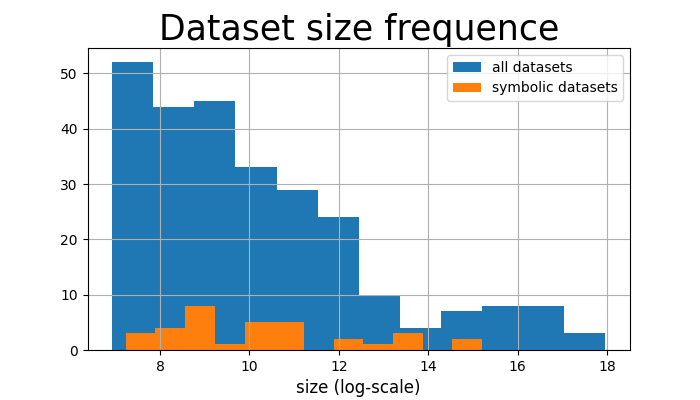
\includegraphics[width=0.5\linewidth]{figures/dataset-size-frequence.png}
  \caption{Size analysis of datasets presented by \cite{UCI}  with more than 1000 instances.
  }
  \label{fig:size}
\end{figure}

%% \subsection{Not really symbolic}
Many encountered \textit{symbolic features} have a latent order as addressed by\cite{OCD}. For example the dataset introduced by  \cite{CarDataset}, which contains cars characteristics, presents a \textit{symbolic feature} ``the size of luggage boot``. This feature often can be ordinaly encoded into a numerical feature following the latent order:

\begin{equation*}
    small \leq med \leq big
\end{equation*}

This remark also applies on binary features, such as boolean ones, that are sometimes recorded as symbolic as in the work of \cite{SPECT} but can directly be treated as numerical. Classical methods on numerical data can applied to those ones.
%%\vfill
These remarks stress the need and the difficulty to correctly handle symbolic features in all machine learning methods, even the gradient-based ones.


\section{Symbolic models and feature encoding}\label{sec:encoding}

% \begin{itemize}
%     \item Maxime \ok ? \no ?
%     \item Thierry \ok ? \no ?
%     \item Victor \ok ? \no ?
% \end{itemize}

%Model optimization through gradient descent is done on a daily basis in Machine Learning where input data can be numerical or symbolic. In this work we focus on symbolic data and adapted models.
\begin{table}[h!]% h asks to places the floating element [h]ere.
  \caption{symbolic data}
  \label{tab:catData}
  \begin{footnotesize}
  \begin{center}
  \begin{tabular}{llc}
    \toprule
    Color & Store & Sales \\
    \midrule
    blue  & Paris    & 14 \\
    pink  & Rome     & 12 \\
    pink  & Rome     & 13 \\
    \dots & \dots    & \dots \\
    blue  & Berlin     & 17 \\
    pink  & Paris     & 8  \\
  \bottomrule
\end{tabular}
\end{center}
\end{footnotesize}
\end{table}

Let us denote ``\catmod`` the set of models that accept symbolic features by design and are numerical , i.e. their parameters can be updated through gradient descent.
By symbolic features, we denote a feature $s$ belonging to an alphabet of $n_{s}$ symbols $\left\{s_1,\cdots, s_{n_{s}} \right\}$, whose cardinality depends on the data. In Table \ref{tab:catData}, color and stores are symbolic features, and pink and blue are symbols, and forms the color alphabet. For example logistic regression introduced by \cite{cox1958regression} belongs to this set of models. 
Wide models described in \cite{wideAndDeep} also correspond to this.
However, Decision Trees do not as they cannot be considered numerical models, but rather ensemble models. Regular neural networks are not \catmod either because they cannot use raw symbolic input data and need to be encoded.


A straightforward \catmod for inputs taken from Table \ref{tab:catData} could be \ref{catModel} and is represented through the graphical representation depicted in Figure \ref{fig:featTokenizerOWN}

\begin{equation}\label{catModel}
    \hat{y} = \mu_{color} \times \gamma_{store}
\end{equation}


\begin{figure*}[h!]
\centering
\begin{tikzpicture}[scale=1]
\begin{scope}[every node/.style={square,thick,draw,minimum size=1cm,fill=green!50,opacity=.2,text opacity=1}]
    \node (Color) at (1,0)  {\tikz\draw[magenta,fill=magenta] (0,0) circle (.9ex);};
\end{scope}

\begin{scope}[every node/.style={square,thick,draw,minimum size=1cm,fill=yellow!50,opacity=.2,text opacity=1}]
    \node (Store) at (5,0) {\small Rome};
\end{scope}

\begin{scope}
    \node (mucolor)  at (1.0,2.8) {$\mu_{color}$};
    \node (gammastore) at (5,2.8)  {$\gamma_{store}$};
\end{scope}

\begin{scope}
    \node (dataColor)  at (1.0,-1) {color};
    \node (data)  at (-2.9,0)    [anchor=west]  {\small data};
    \node (param)  at (-2.9,2)  [anchor=west]    {\small parameters};
    \node (pred)  at (-2.9,4)   [anchor=west]   {\small prediction};
    \node (dataStore)  at (5,-1)    {store};
\end{scope}


\begin{scope}[every node/.style={square,thick,draw,minimum size=1cm,fill=green!50,opacity=.8,text opacity=1}]
    \node (pink) at (1.55,2) %%{\textcolor{magenta}{\mu_{pink}}};
    {\textcolor{magenta}{$\mu_{pink}$}};
    %%{\tikz\draw[magenta,fill=magenta] (0,0) circle (.9ex);};
\end{scope}

\begin{scope}[every node/.style={square,thick,draw,minimum size=1cm,fill=green!50,opacity=.2,text opacity=1}]
    \node (blue) at (0.45,2) 
    {\textcolor{blue}{$\mu_{blue}$}};
    %%{\tikz\draw[blue,fill=blue] (0,0) circle (.9ex);};
\end{scope}

\begin{scope}[every node/.style={square,thick,draw,minimum size=1cm,fill=yellow!50,opacity=.8,text opacity=1}]
    \node (M) at (5,2) {\small \textbf{$\gamma_{Rome}$}};
\end{scope}

\begin{scope}[every node/.style={square,thick,draw,minimum size=1cm,fill=yellow!50,opacity=.2,text opacity=1}]
    \node (S) at (3.75,2) {\small $\gamma_{Paris}$ };
    \node (L) at (6.3,2) {\small $\gamma_{Berlin}$};
\end{scope}

\begin{scope}[every node/.style={square,thick,draw,minimum size=1cm,fill=gray!50,opacity=.2,text opacity=1}]
    \node (y) at (3,4) {$\hat{y}$};
\end{scope}

\begin{scope}[>={Stealth[black]},
              every node/.style={fill=white,circle},
              %%every edge/.style={very thick, color=black}]
              every edge/.style={thin, color=black}]
    \path [->] (Color) edge[draw=black] (pink);
    \path [->] (Store)  edge[draw=black] (M);
    \path [->] (pink)  edge[draw=black] (y);
    \path [->] (M)     edge[draw=black] (y);
    
\end{scope}

\end{tikzpicture}
\caption{\catmod accessing parameters}
\label{fig:featTokenizerOWN}
\end{figure*}


%\begin{figure}[h!]
%\centering
%\begin{tikzpicture}[scale=0.8]
%\begin{scope}[every node/.style={circle,thick,draw,minimum size=1.0cm}]
%\begin{footnotesize}
%    \node (muc) [fill=gray,opacity=.2,text opacity=1] at (1,1) {$\mu_{color}$};
%    \node (gs) at (5,1) {$\gamma_{store}$};
%    \node (y)   at (3,3) {$\hat{y}$} ;
%\end{footnotesize}
%\end{scope}
%\begin{scope}[every node/.style={circle,thick,draw,minimum size=1.0cm,color=white,opacity=0.1,text opacity=1}]
%    \node (*)[color=white]   at (3,2) {\textcolor{black}{*}} ;
%\end{scope}
%
%\begin{scope}[>={Stealth[black]},
%             every node/.style={fill=white,circle},
%              %%every edge/.style={very thick, color=black}]
%              every edge/.style={thick, color=black}]
%    \path [->] (muc) edge[draw=black] (y);
%    \path [->] (gs) edge[draw=black] (y);
%%    \path [->] (F') edge[draw=black]  (P');
%%    \path [->] (P) edge[draw=black, dashed]  (P');
%\end{scope}
%\end{tikzpicture}
%\caption{\catmod}
%\label{fig:catModel}
%\end{figure}

 with $\hat{y}$ the estimated sales. This toy model will be used as an example throughout the paper.

We stress the fact that the \textit{symbolic} aspect applies to the input features: a \catmod can be used for regression, multi-class classification \dots

In this simple model \ref{catModel}, the parameter $\mu_{color}$ has thus a value for each color, and we aim to find the best ones in order to have a good predictive model. One of the main techniques to do that is gradient descent. Partly due to the very large amount of data often encountered in practice, \textit{stochastic} gradient descent is used. However, applying \textit{stochastic} gradient descent on \catmod raises an issue as common gradient update techniques are not designed for symbolic features: not every symbol of a symbolic feature is present in every observation of a dataset while regular numerical models assume that every feature is present on every observation. We propose an updated version of gradient estimation used to update parameters. Its specificity is to take into account the symbolic features. This paper links work on sparse gradient estimator and \ohe symbolic data that leads to a sparse but structured gradient.






\catmod have to deal with numbers as parameters, not symbols. Symbolic data require a numerical embedding before they can be given as input.




Many possible encodings exist:
\begin{fleqn}
\begin{align*}
    &\bullet \text{ordinal encoding} &&\bullet \text{leave-one-out encoding}\\
    &\bullet \text{\ohe}             &&\bullet \text{positional encoding} \quad \quad \\
    &\bullet \text{binary encoding}  &&\bullet \text{\dots}\\
    &\bullet \text{target encoding}  && \\
\end{align*}
\end{fleqn}

% \begin{multicols*}{2}
% \begin{itemize}
%     \setlength\itemsep{-0.4em}
%     \item ordinal encoding
%     \item \ohe
%     \item binary encoding
%     \item target encoding
% \end{itemize}

% \begin{itemize}
%     \setlength\itemsep{-0.4em}
%     \item leave-one-out encoding 
%     \item positional encoding
%     \item \dots
% \end{itemize}
% \end{multicols*}

% \begin{itemize}
%     \setlength\itemsep{-0.4em}
%     \item ordinal encoding
%     \item \ohe
%     \item binary encoding
%     \item target encoding
%     \item leave-one-out encoding 
%     \item positional encoding
%     \item \dots
% \end{itemize}

No universally good method of encoding exists and choice should always rely on data (alphabet cardinality, relationships between them \dots). In the following we will focus on \ohe because it is precisely what is done in a \catmod. Model \ref{catModel} \ohe is depicted in Equation \ref{eq:muEncoding} and Figure \ref{fig:featTokenizerOWN}.


\ohe a symbolic variable with cardinality n is performed by creating n binary vectors for each occurrence of the symbol. If there are few symbols, there are only a few newly created columns. On data stored in Table \ref{tab:catData}, \ohe the feature \textit{Color} creates the features $is_{blue}$ and $is_{pink}$. Thus \ohe is adapted to low cardinality features. Otherwise one might face the curse of dimensionality as described in \cite{curse}. Moreover, symbols present in the testing dataset but unseen in the training dataset are incompatible with \ohe as it makes the assumption that all symbols are present in the training dataset; the data is pre-processed according to them. Text encoding as presented in \cite{sundae} or \cite{textClassification} represents sentences in a latent space, as two different ones might have a very similar meaning and thus a very close representation in the latent space. This does not apply on symbolic data where each symbol has a very specific meaning.
When those adequate conditions are not met, other encodings (such as leave-one-out) should be preferred. 


%%%%%%%%%%%%%%%%%%%%%%%%%%%%%%%%
%%%%%%%%%%%%%%%%%%%%%%%%%%%%%%%%
% \newpage
% \begin{figure}[h!]
% \centering
% \begin{tikzpicture}[scale=0.8]
% \begin{scope}[every node/.style={circle,thick,draw,minimum size=1.0cm}]
% \begin{footnotesize}
%     \node (mublue) at (1,0)     {$\mu_{blue}$};
%     \node (isb)    at (3,0)     {$is_{blue}$};
%     \node (mupink) at (5,0)     {$\mu_{pink}$};
%     \node (isp)    at (7,0)     {$is_{pink}$};
%     \node (mub)   [fill=blue,opacity=.2,text opacity=1] at (2.5,2.5) {$\mu_b$};
%     \node (mup)   [fill=magenta,opacity=.2,text opacity=1] at (4.5,2.5) {$\mu_p$};
%     \node (mu)    [fill=gray,opacity=.2,text opacity=1] at (5,4.5)   {$\mu$};
    
%     \node (gs)     at (7,2)     {$\gamma_{size}$};
%     \node (y)      at (6,6.3)     {$\hat{y}$} ;
%     \end{footnotesize}
% \end{scope}

% \begin{scope}[every node/.style={circle,thick,draw,minimum size=1.0cm,color=black,opacity=0.0,text opacity=1}]
%     \node (*)  at (5.8, 5.35)  {*} ;
%     \node (+)  at (4.5, 3.65) {+} ;
%     \node (*b) at (2.3, 1.6)  {*} ;
%     \node (*p) at (4.9, 1.6)  {*} ;
% \end{scope}

% \begin{scope}[>={Stealth[black]},
%               every node/.style={fill=white,circle},
%               %%every edge/.style={very thick, color=black}]
%               every edge/.style={thick, color=black}]
%     \path [->] (mublue) edge[draw=black] (mub);
%     \path [->] (mupink) edge[draw=black] (mup);
%     \path [->] (isb)    edge[draw=black] (mub);
%     \path [->] (isp)    edge[draw=black] (mup);
%     \path [->] (mup)    edge[draw=black] (mu) ;
%     \path [->] (mub)    edge[draw=black] (mu) ;
%     \path [->] (mu)     edge[draw=black] (y)  ;
    
%     \path [->] (gs) edge[draw=black] (y);
% \end{scope}
% \end{tikzpicture}
% \caption{One-Hot encoded \catmod}
% \label{fig:catModelOneHot}
% \end{figure}

% Of course this encoding is also done for $\gamma_{size}$.
% \\
% \textbf{\textcolor{red}{OR}}
%%%%%%%%%%%%%%%%%%%%%%%%%%%%%%%%
%%%%%%%%%%%%%%%%%%%%%%%%%%%%%%%%





Interpretability of the model is fundamental as explained by \cite{Stop} especially in high-stake contexts such as disease diagnostics, where explanability of the result is expected for the human expert to take his final decision.
In this direction, using \ohe  is crucial. Having parameters directly related to the application semantic by giving access to their relation with the input symbols is a requirement for the design of white-box models. In model \ref{catModel}, $\mu_{blue}$ ($\mu_{pink}$ respectively) has a valuable meaning: this is the impact of the blue (pink respectively) color on the sales. Parameters value not only serve model prediction quality, they are also \textit{interpretable}.  On Model \ref{catModel}, $\mu_{blue} >\mu_{pink}$ means that the blue color sells better than the pink one. Not only is the prediction of the model explainable, but the model itself conveys meaning, even without inputs.

Leave-one-out encoding turns the symbolic feature into \textbf{one} numerical feature. This has several advantages (no curse of dimensionality for example) but gives no directly interpretable parameters.

\ohe leads to sparse but structured data by construction. Gradient descent on sparse data is an extensively studied subject: \cite{GDsparseData} \cite{FastLearningSparse}; \cite{LinearLearningSparseData}; \cite{SparseOnlineLearning} \dots The following also applies to sparse but structured data. As \ohe is not suited for high-cardinality symbolic “sparse” features we exclude such feature from the following, which is not restrictive for domains such as health or supply chain.

\section{Problem description}


% \begin{itemize}
%     \item Maxime \ok ? \no ?
%     \item Thierry \ok ? \no ?
%     \item Victor \ok ? \no ?
% \end{itemize}

In this section we present the  problems encountered with using one hot encoding and then illustrate it in the online learning set up.


\subsection{Notation}\label{notations}

We consider the supervised learning set up with a given set of training labeled data $\mathcal{Z} = \{ z_i = (X_i; y_i); i = 1 \dots  n \}$, with the feature
vectors $X_i \in \mathbb{R}^p$ and the scalar targets $y_i \in \mathbb{R}$. Each one of the $p$ components of the feature vectors is related to one of the $p$ symbols $\{ s_k\}_{k \leq p}$:

\begin{equation} \label{eq:symbol}
    \forall (X_i, \cdot) \in \mathcal{Z} \quad \forall k \leq p \quad X_i \text{ corresponds to } s_k \iif X_{i}^k \neq 0
\end{equation}

We aim to find the best parameter $\theta^\star \in \mathbb{R}^m$ ($m \geq p$) to minimize the loss $F_{\theta^\star}$ on the whole dataset:

\begin{align*}
    f: \quad &\Theta \times \mathcal{Z} \longrightarrow \mathbb{R}\\
            &\theta, (X,y) \longrightarrow  f_{\theta}(X,y)
\end{align*}

\begin{align*}
\theta^\star &= \underset{\theta}{\argmin} \quad F_\theta\\
             &= \underset{\theta}{\argmin} \sum_{X,y \in \mathcal{Z}} f_\theta (X,y)\\
             &= \underset{\theta}{\argmin} \sum_{i=1\dots n} f_\theta (X_i,y_i)
\end{align*}

This notation is generic and includes sparse data in general. One-hot encoded data is a specific case of sparse data.














%%%%%%%%%%%%%%%%%%%%%%%%%%%%%%%%%%%%%%%%%%%%%%%%%%%%%%%%%%%%%%%%%%%%%%%%%%%%%%%%%%%%%%%%%
%%%%%%%%%%%%%%%%%%%%%%%%%%%%%%%%%%%%%%%%%%%%%%%%%%%%%%%%%%%%%%%%%%%%%%%%%%%%%%%%%%%%%%%%%
%%%%%%%%%%%%%%%%%%%%%%%%%%%%%%%%%%%%%%%%%%%%%%%%%%%%%%%%%%%%%%%%%%%%%%%%%%%%%%%%%%%%%%%%%
%%%%%%%%%%%%%%%%%%%%%%%%%%%%%%%%%%%%%%%%%%%%%%%%%%%%%%%%%%%%%%%%%%%%%%%%%%%%%%%%%%%%%%%%%
%%%%%%%%%%%%%%%%%%%%%%%%%%%%%%%%%%%%%%%%%%%%%%%%%%%%%%%%%%%%%%%%%%%%%%%%%%%%%%%%%%%%%%%%%
%%%%%%%%%%%%%%%%%%%%%%%%%%%%%%%%%%%%%%%%%%%%%%%%%%%%%%%%%%%%%%%%%%%%%%%%%%%%%%%%%%%%%%%%%
%%%%%%%%%%%%%%%%%%%%%%%%%%%%%%%%%%%%%%%%%%%%%%%%%%%%%%%%%%%%%%%%%%%%%%%%%%%%%%%%%%%%%%%%%

\begin{figure*}
\centering
\begin{subfigure}{0.48\linewidth}
\centering
%%\begin{figure}[h!]
%%\centering
\begin{tikzpicture}[scale=0.7]

\draw (-0.9,11) --(-1,11) -- (-1,0) -- (-0.9,0) ;
\draw (0.9,11) --(1,11) -- (1,0) -- (0.9,0) ;

\node (x1)   at (0,10)  {$x_1$};
\node (x2)   at (0,9)  {$x_2$};
\node (x3)   at (0,8)  {$x_3$};
\node (x4)   at (0,7)  {$x_4$};
\node (x5)   at (0,6)  {$x_5$};
\node (xdot) at (0,4)  {\dots};
\node (xpm1) at (0,2)  {$x_{p-1}$};
\node (xp)   at (0,1)  {$x_p$};

\node (feat1) at (-2,9)   {\textcolor{orange}{$feat_1$}};
\node (feat2) at (-2,6.5) {\textcolor{black}{$feat_2$}};
\node (feat3) at (-2,1.5) {\textcolor{green}{$feat_C$}};



\node (X)     at (-1.9,4) {\Large $X = $};
\node (Theta) at (5.7,4)  {\Large $ = \theta $};


\draw [decorate, decoration = {brace,mirror}, color=orange] (-0.6,10.2) -- (-0.6,7.8);
\draw [decorate, decoration = {brace,mirror}, color=black]  (-0.6,7.2)  -- (-0.6,5.8);
\draw [decorate, decoration = {brace,mirror}, color=green]  (-0.6,2.2)  -- (-0.6,0.8);


\draw (3.1,11) --(3,11) -- (3,-2) -- (3.1,-2) ;
\draw (4.9,11) --(5,11) -- (5,-2) -- (4.9,-2) ;

\node (theta1)   at (4,10)   {$\theta_1$};
\node (theta2)   at (4,9)    {$\theta_2$};
\node (theta3)   at (4,8)    {$\theta_3$};
\node (theta4)   at (4,7)    {$\theta_4$};
\node (theta5)   at (4,6)    {$\theta_5$};
\node (theta6)   at (4,5)    {$\theta_6$};
\node (thetadot) at (4,2)    {\dots};
\node (thetaM)   at (4,-1)  {$\theta_M$};


\path [->] (x1) edge[draw=black] (theta1);
\path [->] (x1) edge[draw=black] (theta2);
\path [->] (x1) edge[draw=black] (theta3);
\path [->] (x2) edge[draw=black] (theta4);
\path [->] (x3) edge[draw=black] (theta5);
\path [->] (x3) edge[draw=black] (theta6);
\path [->] (xp) edge[draw=black] (thetaM);

\draw [decorate, decoration = {brace,mirror}, color=orange]  (4.5,4.8) -- (4.5,10.2) ;

\end{tikzpicture}
\caption{Generic n  otations}
\label{fig:generalnotations}
\end{subfigure}
\begin{subfigure}{0.48\linewidth}

%%\begin{figure}[h!]
%%\centering
\begin{tikzpicture}[scale=0.7]

\draw (-0.9,11) --(-1,11) -- (-1,4) -- (-0.9,4) ;
\draw (0.9,11) --(1,11) -- (1,4) -- (0.9,4) ;

\node (blue)  at (0,10) {\small $is_{blue}$};
\node (pink)  at (0,9)  {\small $is_{pink}$};
\node (Paris)     at (0,7)  {\small $is_{Paris}$};
\node (Rome)     at (0,6)  {\small $is_{Rome}$};
\node (Berlin)     at (0,5)  {\small $is_{Berlin}$};

\node (color) at (-2,9.5)   {\small $color$};
\node (store) at (-2,6) {\small $store$};


\node (X)     at (-1.9,8) {\Large $X = $};
\node (Theta) at (5.7,8)  {\Large $ = \theta $};


\draw [decorate, decoration = {brace,mirror}] (-1.1,10.2) -- (-1.1,8.8);
\draw [decorate, decoration = {brace,mirror}] (-1.1,7.2) -- (-1.1,4.8);


\draw (3.1,11) --(3,11) -- (3,4) -- (3.1,4) ;
\draw (4.9,11) --(5,11) -- (5,4) -- (4.9,4) ;

\node (mublue)   at (4,10)   {$\mu_{blue}$};
\node (mupink)   at (4,9)    {$\mu_{pink}$};

\node (muparis)  at (4,7)    {\small $\gamma_{Paris}$};
\node (murome)   at (4,6)    {\small $\gamma_{Rome}$};
\node (muberlin) at (4,5)    {\small $\gamma_{Berlin}$};


\path [->] (blue)   edge[draw=black] (mublue);
\path [->] (pink)   edge[draw=black] (mupink);
\path [->] (Paris)  edge[draw=black] (muparis);
\path [->] (Rome)   edge[draw=black] (murome);
\path [->] (Berlin) edge[draw=black] (muberlin);


\end{tikzpicture}
\caption{Notations applied to Model \ref{catModel}}
\label{fig:notationsModel1}
\end{subfigure}
\caption{Notations}
\label{fig:notations}
\end{figure*}


Figure \ref{fig:notations} illustrates the formal definition. In Figure \ref{fig:generalnotations}, $\{ \theta_1 ;  \theta_2 ;  \theta_3 ;  \theta_4 ;  \theta_5 ;  \theta_6 ; \}$ are related to the first feature $\textcolor{orange}{feat_1}$. On Model \ref{catModel}, such notations give Figure \ref{fig:notationsModel1}.
%%%%%%%%%%%%%%%%%%%%%%%%%%%%%%%%%%%%%%%%%%%%%%%%%%%%%%%%%%%%%%%%%%%%%%%%%%%%%%%%%%%%%%%%%
%%%%%%%%%%%%%%%%%%%%%%%%%%%%%%%%%%%%%%%%%%%%%%%%%%%%%%%%%%%%%%%%%%%%%%%%%%%%%%%%%%%%%%%%%
%%%%%%%%%%%%%%%%%%%%%%%%%%%%%%%%%%%%%%%%%%%%%%%%%%%%%%%%%%%%%%%%%%%%%%%%%%%%%%%%%%%%%%%%%
%%%%%%%%%%%%%%%%%%%%%%%%%%%%%%%%%%%%%%%%%%%%%%%%%%%%%%%%%%%%%%%%%%%%%%%%%%%%%%%%%%%%%%%%%
%%%%%%%%%%%%%%%%%%%%%%%%%%%%%%%%%%%%%%%%%%%%%%%%%%%%%%%%%%%%%%%%%%%%%%%%%%%%%%%%%%%%%%%%%
%%%%%%%%%%%%%%%%%%%%%%%%%%%%%%%%%%%%%%%%%%%%%%%%%%%%%%%%%%%%%%%%%%%%%%%%%%%%%%%%%%%%%%%%%
%%%%%%%%%%%%%%%%%%%%%%%%%%%%%%%%%%%%%%%%%%%%%%%%%%%%%%%%%%%%%%%%%%%%%%%%%%%%%%%%%%%%%%%%%
%%%%%%%%%%%%%%%%%%%%%%%%%%%%%%%%%%%%%%%%%%%%%%%%%%%%%%%%%%%%%%%%%%%%%%%%%%%%%%%%%%%%%%%%%
%%%%%%%%%%%%%%%%%%%%%%%%%%%%%%%%%%%%%%%%%%%%%%%%%%%%%%%%%%%%%%%%%%%%%%%%%%%%%%%%%%%%%%%%%
%%%%%%%%%%%%%%%%%%%%%%%%%%%%%%%%%%%%%%%%%%%%%%%%%%%%%%%%%%%%%%%%%%%%%%%%%%%%%%%%%%%%%%%%%
%%%%%%%%%%%%%%%%%%%%%%%%%%%%%%%%%%%%%%%%%%%%%%%%%%%%%%%%%%%%%%%%%%%%%%%%%%%%%%%%%%%%%%%%%
%%%%%%%%%%%%%%%%%%%%%%%%%%%%%%%%%%%%%%%%%%%%%%%%%%%%%%%%%%%%%%%%%%%%%%%%%%%%%%%%%%%%%%%%%
%%%%%%%%%%%%%%%%%%%%%%%%%%%%%%%%%%%%%%%%%%%%%%%%%%%%%%%%%%%%%%%%%%%%%%%%%%%%%%%%%%%%%%%%%




\subsection{Gradient descent with symbolic variables}\label{sec:motication}
Classical stochastic gradient descent relies on an unbiased gradient's estimator. Rather than using the complete gradient on all observations, observations are divided into \textit{batches} and the gradient is estimated on those:
\begin{align}
\nabla F &=  \frac{1}{n} \sum_{obs} \nabla f_{obs}  = \frac{1}{n} \sum_{i \leq n} \nabla_{\theta} f(X_i, y_i)     \\
         &= \frac{1}{n} \sum_{batch} \quad \sum_{obs \in batch} \nabla f_{obs}
\end{align}
In particular, this makes sense on large datasets where computing the exact full (i.e. on all observations) gradient might be very expensive.
The accumulated gradient is then divided by the size of the batch to get the gradient mean. Gradient descent techniques succeed in finding a minimum, notably because this the gradient estimator is unbiased. 

Regarding \catmod, we can highlight the fact that not every symbolic parameter is affected by every observation. For example in model \ref{catModel} $\mu_{blue}$ is only used on observations that concern a blue product. By construction via \ohe each observation concerns one and only one symbol for each symbolic feature. Applying Gradient descent in a batch mode to estimate the gradient gives a biased estimator. This issue is exacerbated on a batch that does not include a symbol. In this instance, the gradient does not even make sense.

\begin{align}
\nabla_{\mu_{blue}} F &= \frac{1}{n} \sum_{obs} \nabla_{\mu_{blue}} f_{obs}\\
         &= \frac{1}{n} \sum_{batch} \underset{color(obs) = blue}{\sum_{{obs \in batch}}} \nabla_{\mu_{blue}} f_{obs}
\label{eq:gradientDecomp}
\end{align}


What would be the parameter's gradient of a symbol that is not present at all in the dataset? What would be the gradient of $\mu_{red}$ in Model \ref{catModel} with no red products? $\{ obs \in batch | color(obs) = blue \}$ from Equation \ref{eq:gradientDecomp} might be empty, and in this case parameters related to the \textit{blue} symbol are not present. And \mainContrib. Thanks to \ohe, we have prior info on the data and the gradient. With an observation that does not concerns the symbol $s_k$, we know \textbf{for a fact} that the gradient of its related parameters will be numerically zero. Thus this numerically zero gradient does not bring any information, it should not be used for parameters updates.

\begin{align*}
    &\mu_{color} = \mu_{blue} \times is_{blue} + \mu_{pink} \times is_{pink} \numberthis \label{eq:muEncoding} \\
    &\frac{\partial\mu_{color}}{\partial\mu_{blue}}\mid_{color = pink} = 0\\
    &\frac{\partial\mu_{color}}{\partial\mu_{pink}}\mid_{color = blue} = 0
\end{align*}


This issue  especially concerns under-represented symbols and small batches. The smallest the symbol cardinality and the smallest the batch, the highest probability to not be included in the batch. When a symbol is not present in the batch, we state that its related parameters should not be modified. To support this idea, an online learning (i.e. with batch size of 1) example is presented in Section \ref{tinyBatch}. Many descent techniques\footnote{not all, see \cite{biased} for example} \cite{RAD} such as  \cite{rebar} or \cite{unbmixture} that rely on an estimator of the gradient use an unbiased estimator of the gradient. \cite{BachProof} proves that it is a sufficient condition for convergence in the convex setting. Here the gradients of the symbolic parameters are somehow biased. 



\ohe should not be part of the model (see Equation \ref{eq:muEncoding}). It is a way to deal with symbolic data as positional encoding is not integrated to Transformers \cite{attentionIsAllYouNeed}. As it is not part of the model itself, it should not infer on model's parameters updates.


\secondContrib.

\subsection{Online Gradient descent}\label{tinyBatch}
Let's consider the case of batches of size 1 also called online learning. It means that observations are taken one by one. In Model \ref{catModel} Each observation concerns one and only one \textit{color} and one and only one \textit{store}.



\begin{table}[h]% h asks to places the floating element [h]ere.
  \caption{symbolic data}
  \begin{footnotesize}
  \begin{center}
  \begin{tabular}{llc}
    \toprule
    Color & Store & Sales \\
    \midrule
    blue  & Paris & 14 \\
    pink  & Rome  & 12 \\
    \textcolor{magenta}{\textbf{pink}}  & \textcolor{magenta}{\textbf{Rome}}     & \textcolor{magenta}{\textbf{13}} \\
    \dots & \dots & \dots \\
    blue  & Berlin    & 17 \\
    pink  & Paris     & 8  \\
  \bottomrule
\end{tabular}
\end{center}
\end{footnotesize}
\end{table}


In this case it is logical to only update the parameters of the concerned symbol. The gradients of the parameters of the unconcerned symbols \textbf{do not exist}. And \mainContrib.

This logical behaviour for online learning should be generalized to bigger batches.

\subsection{Comparison with common optimizer}

Adagrad introduced by \cite{Adagrad} is an optimizer to update parameters through gradient descent; the learning rate is parameter's history dependant:

\begin{equation*}
    \theta_{t,j} = \theta_{t-1,j} - \frac{\alpha}{\sqrt{\underset{\tau = 1}{\overset{t}{\sum}} \nabla_{\theta_{j,\tau}}f^2}} \nabla_{\theta_{j,t}}f 
\end{equation*}

Adagrad performs smaller updates for parameters associated with frequently occurring symbols, and larger updates for parameters associated with infrequent symbols. It has been designed to support sparse input such as one encoded data. Indeed an infrequent symbol (associated to $\theta_{j,t}$) will have a relatively small gradient history$\underset{\tau = 1}{\overset{t}{\sum}} \nabla_{\theta_{j,\tau}}f^{2}_{\tau,j}$ as $\nabla_{\theta_{j,\tau}}f$ is often zero, which leads to a relatively big learning rate. To our knowledge it is one of the very few optimizer widely used that intrinsically take into account sparse data.

Many gradient-based models as \cite{OptimizerReview} updates their parameters with Adam \cite{adam} or modified versions of it \cite{adamw} \cite{nadam} as an optimizer. We can state that Adam is one of the default optimizer in Machine Learning in general. To simplify, with Adam, parameters are updated with their \textit{momentum} taken into account. Using batches on symbolic data leads to "slow down" parameters' \textit{momentum} if not present in the batch and follow their \textit{momentum} for many batches if not present in consecutive ones. With the original Adam notation, a zero gradient gives:


\begin{align*}
    m_{t} &= \beta_1 \times m_{t-1} \\
    v_{t} &= \beta_2 \times v_{t-1} \\
    \theta_t &= \theta_{t-1} - \frac{\alpha}{1 - \beta_1^t} \frac{m_t}{\epsilon + \sqrt{\frac{v_t}{1-\beta_2^t}}}
\end{align*}

If a symbol is rarely present in batches, its related parameter will \textit{follow} its \textit{momentum} (created on batches where it is present) on batches where it is absent. This update does not make any sense for parameters that have been unused during the batch.












\section{Deep Learning}\label{deepLearning}

% \begin{itemize}
%     \item Maxime \ok ? \no ?
%     \item Thierry \ok ? \no ?
%     \item Victor \ok ? \no ?
% \end{itemize}



Most deep architectures are built to support numerical data such as image or audio but \ohe approach has already been applied by \cite{RevisitingDeepForTabular} for example and is called \textit{Feature Tokenizer}. Applying \textbf{one-hot-encoding} to feed neural networks is theoretically equivalent to use a different network for each symbol. We illustrate that on a dense linear layer as depicted in Figures \ref{fig:catModelOneHot}. This use of different networks for each symbols raises the issue depicted in \ref{sec:motication} when used with \textit{batch} during training. Gradient estimation done by \textit{batch} implies that the parameters are used on every observation, which totally makes sense for classical Deep Learning (i.e. with no one-hot encoded data). If a symbol is not present in a \textit{batch}, it means that there is no accumulated gradient, which is different than accumulated gradient is zero.



\begin{figure*}
\centering
\begin{subfigure}{0.48\linewidth}
\centering
\begin{tikzpicture}[scale=0.8]
\begin{scope}[every node/.style={square,thick,draw,minimum size=0.8pt}]
\begin{footnotesize}
    \node (num1) at (0,8)  {};
    \node (num1bis) at (2,8)  {};
    \node (num2) at (0,5.5)   {};
    \node (num3) at (0,4)   {};
    \node (hidden1) [color=red] at (4,5)     {};
    \node (hidden2) [color=red] at (4,7)     {};
\end{footnotesize}
\end{scope}
\begin{scope}[every node/.style={square,thick,draw,minimum size=2.05cm}]
\begin{small}
    \node (container) [color=blue] at (1,8) {};
\end{small}
\end{scope}
\begin{scope}[>={Stealth[black]},
              every node/.style={fill=white,circle},
              every edge/.style={thin, color=black}]
    \path [->] (num1) edge[draw=black, dashed] (num1bis);
    \path [->] (num1bis) edge[draw=black] (hidden1);
    \path [->] (num1bis) edge[draw=black] (hidden2);
    \path [->] (num2) edge[draw=black, dashed] (hidden1);
    \path [->] (num2) edge[draw=black, dashed] (hidden2);
    \path [->] (num3) edge[draw=black, dashed] (hidden1);
    \path [->] (num3) edge[draw=black, dashed] (hidden2);
\end{scope}
\end{tikzpicture}
\caption{Dense Layer}
\label{fig:catModelOneHotPART1}
\end{subfigure}
\begin{subfigure}{0.48\linewidth}
\centering
\begin{tikzpicture}[scale=0.6]
\begin{scope}[every node/.style={square,thick,draw,minimum size=1.2pt}]
%%    \node (in) at (-1.2,6)  {};
    \node (hidden2) at (4,5) {};
    \node (hidden1) at (4,7) {};
\end{scope}

\begin{scope}[every node/.style={square,thick,draw,minimum size=25pt,fill=gray,opacity=.2,text opacity=1}]
\begin{footnotesize}
    \node (A) at (0,8)  {$is_{blue}$};
    \node (B) at (0,6)  {$is_{pink}$};
    \node (C) at (0,4)  {$is_{green}$};
\end{footnotesize}
\end{scope}

\begin{scope}[every node/.style={square,thick,draw,minimum size=4cm}]
    \node (container) [color=blue] at (1.7,6) {};
\end{scope}
\begin{scope}[every node/.style={square,thick,draw,minimum size=1.2pt}]
    \node (out1) [color=red] at (7,6) {};
    \node (out2) [color=red] at (7,2) {};
\end{scope}

\begin{scope}[>={Stealth[black]},
              every node/.style={fill=white,circle},
              %%every edge/.style={very thick, color=black}]
              every edge/.style={thin, color=black}]
    \path [->] (A) edge[draw=black, dashed] (hidden1);
    \path [->] (A) edge[draw=black, dashed] (hidden2);
    \path [->] (B) edge[draw=black, dashed] (hidden1);
    \path [->] (B) edge[draw=black, dashed] (hidden2);
    \path [->] (C) edge[draw=black, dashed] (hidden1);
    \path [->] (C) edge[draw=black, dashed] (hidden2);
    \path [->] (hidden1) edge[draw=black] (out1);
    \path [->] (hidden2) edge[draw=black] (out2);

\end{scope}
\end{tikzpicture}
\caption{\ohe of a dense layer}
\label{fig:catModelOneHotPART2}
\end{subfigure}
\begin{subfigure}{0.5\linewidth}
\centering
\begin{tikzpicture}[scale=0.6]
\begin{scope}[every node/.style={square,thick,draw,minimum size=1.2pt}]
%%    \node (in) at (-1.2,6)  {};
    \node (hidden2) at (4,5) {};
    \node (hidden1) at (4,7) {};
\end{scope}

\begin{scope}[every node/.style={square,thick,draw,minimum size=25pt,fill=gray,opacity=.2,text opacity=1}]
\begin{footnotesize}
    \node (A) at (0,8)  {$is_{blue}$};
    \node (B) at (0,6)  {$is_{pink}$};
    \node (C) at (0,4)  {$is_{green}$};
\end{footnotesize}
\end{scope}

\begin{scope}[every node/.style={square,thick,draw,minimum size=4cm}]
    \node (container) [color=blue] at (1.7,6) {};
\end{scope}
\begin{scope}[every node/.style={square,thick,draw,minimum size=1.2pt}]
    \node (out1) [color=red] at (7,6) {};
    \node (out2) [color=red] at (7,2) {};
\end{scope}

\begin{scope}[>={Stealth[black]},
              every node/.style={fill=white,circle},
              %%every edge/.style={very thick, color=black}]
              every edge/.style={thin, color=black}]
    \path [->] (A) edge[draw=black, dashed] (hidden1);
    \path [->] (A) edge[draw=black, dashed] (hidden2);
    \path [->] (B) edge[draw=black, dashed] (hidden1);
    \path [->] (B) edge[draw=black, dashed] (hidden2);
    \path [->] (C) edge[draw=red, dashed] (hidden1);
    \path [->] (C) edge[draw=red, dashed] (hidden2);
    \path [->] (hidden1) edge[draw=red] (out1);
    \path [->] (hidden2) edge[draw=red] (out2);

\end{scope}
\end{tikzpicture}
\caption{dense layer relative to she \textit{green} symbol}
\label{fig:catModelOneHotPART2}
\end{subfigure}

\caption{\ohe for neural networks}
\label{fig:catModelOneHot}
\end{figure*}







\section{Solution: \tecname}


% \begin{itemize}
%     \item Maxime \ok ? \no ?
%     \item Thierry \ok ? \no ?
%     \item Victor \ok ? \no ?
% \end{itemize}

With all we've discussed, the solution is straight forward and very easy to implement.

%%%%%%%%%%%%%%%%%%%
% Let \catn{k} be the set of symbol groups for the $k^{th}$ feature and $\theta_{m}$ a symbolic parameter of the symbol $A_j$. With the notations from \ref{notations}: $\sum J_k = p$

% In our example from table \ref{tab:catData} $\{ A_j \} = \{ blue ; pink \}$ and $\theta_m = \mu_{blue}$.

%%%%%%%%%%%%%%%%%%%%%%


%% \subsection{Do not update unconcerned parameters}\label{sec:DoNothing}
If $\{symbol(obs) = s_k / obs \in batch\}$ is empty, parameters related to the $s_k$ symbol should \textbf{not} be updated. Indeed \mainContrib. The proposed gradient estimator thus make the difference between a zero gradient and a non-present gradient. Then one needs to count each symbol uses and to apply the unbiased gradient. Counting symbol uses allow us to compute unbiased gradient. Then:


\begin{align*} 
\ntm F &= \frac{\partial F}{\partial \theta_{m}}\\
 &= \sum_{batch} \sum_{obs \in batch} \ntm f(obs) \\ 
 &= \sum_{batch} \sum_{\underset{obs \in s_k}{obs \in batch}} \ntm f(obs)
\end{align*}
$S_k = \{obs \in batch / symbol(obs) = s_k \} $

So one needs  to divide the accumulated gradient by the cardinality of $S_k = \{obs \in batch / symbol(obs) = s_k \} $. If this set is empty, parameters related to the $s_k$ symbol should not be updated. Again \mainContrib. This is presented in Algorithm \ref{alg:DivideByTheGood}.



\begin{algorithm}
\caption{\tecname}\label{alg:DivideByTheGood}
\begin{algorithmic}[5]
                
\Require $\mathcal{Z}$: data
\Require $update(\cdot  , \cdot  )$: chosen optimizer
\Require $\theta_0$: Initial parameter vector 
\State $t \gets 0$
\While{$\theta_t$ not converged}
    $t \gets t + 1$
    \State Divide $Z$ in $Batches$
    \For{batch $\in$ Batches}
        \For{symbol $\in$ Alphabet}    
            \State $c_{symbol} \gets 0$
        \EndFor
        \State $\textbf{g} \gets \vec{0}$
        \For{X, y $\in$ batch}
            \State $c_{symbol(X)} \gets c_{symbol(X)} + 1$
            \State Compute $\nabla_{\theta_{t-1}} f_{\theta_{t-1}}(X)$ thanks to $y$
            \State $\textbf{g} \gets \textbf{g} + \nabla_{\theta_{t-1}} f_{\theta_{t-1}}(X)$ \Comment{\textbf{\textcolor{blue}{\small accumulate gradient}}}
        \EndFor
        \State $\theta_{t} \gets \theta_{t-1}$
        \For{$symbol \in Alphabet$}
            \If{$c_{symbol} > 0 $}  \Comment{\textcolor{blue}{\small \mainContrib}}
                \State $\theta_{t, symbol} \gets update(\theta_{t-1, symbol}, \frac{1}{c_{symbol}}\textbf{g}_{symbol})$ \Comment{\textbf{\textcolor{blue}{\small scaled gradient}}}
            \EndIf
        \EndFor
    \EndFor 
\EndWhile
\end{algorithmic}
\end{algorithm}



%% \subsection{What does it minimize}

% \TODO : harmonize notations\\

% \TODO : enlever le $\frac{1}{\# cat}$ pour être iso avec ce qu'on a écrit plus haut.\\

% \TODO : si les catégories ont les mêmes tailles alors c'est la même chose ! elles forment une partition et $\#C$ est toujours le même.\\



% \begin{equation}
%     F(x) = \frac{1}{\# Symbols} \sum_{symbol} \sum_{obs \in \{ obs | s(obs) = symbol \} = S} \frac{1}{\# S} loss_x (obs)
% \end{equation}


% \begin{equation*}
%     f_{\binom{M}{m}}(x) = \frac{1}{\# Symbols} \sum_{symbol} \sum_{obs \in = S \cap \binom{M}{m}} \frac{1}{\# S^m} loss_x (obs)
% \end{equation*}

With the current notations:



\begin{equation}\label{eq:realLoss}
    F_{\theta} = \frac{1}{p} \summ{k=1}{p} \sum_{X,y \in S_k}  \frac{1}{\# S_k} f_{\theta} (X, y)
\end{equation}

With such loss objective function, drawing random observations in $\mathcal{Z}$ does not give an unbiased gradient estimator.
\begin{equation*}
    F_{\binom{\mathcal{Z}}{m} \theta} = \frac{1}{p} \summ{k=1}{p} \sum_{X,y \in S_k \cap \binom{\mathcal{Z}}{m}}  \frac{1}{\#[ S_k \cap \binom{\mathcal{Z}}{m}]} f_{\theta} (X, y)
\end{equation*}


$F_{\binom{\mathcal{Z}}{m} \theta}$ is a random estimator of $F_{\theta}$ where $m$ observations (over the $\mathcal{Z}$) are uniformly drawn. It is the estimator used by Algorithm \ref{alg:DivideByTheGood}. This estimator is unbiased, proof can be found in appendices \ref{theorem:unbiased}:

\begin{equation*}
    \esp{\nabla F_{\binom{\mathcal{Z}}{m}}} = \nabla F_{\theta}
\end{equation*}

Which is a sufficient condition for convergence in the convex setting \cite{BachProof}.

 
The loss function depicted in equation \ref{eq:realLoss} seems similar to loss used for classification with unbalanced \textbf{output} categories. Let recall that what we propose here is different as we consider unbalanced \textbf{input} symbols. 

In the case where symbol groups have same size $C$ then the objective function resumes to:

\begin{align*}
    F_{\theta} &= \frac{1}{p}            \summ{k=1}{p} \sum_{X,y \in s_k} \frac{1}{\# s_k} f_{\theta} (X, y)\\
               &= \frac{1}{p}            \summ{k=1}{p}  \frac{1}{C} \sum_{X,y \in s_k}       f_{\theta} (X, y)\\
               &= \frac{1}{p \times C}   \sum_{X,y \in Z}                                      f_{\theta} (X, y)\\
                &= \frac{1}{\mathcal{Z}} \sum_{X,y \in Z}                                      f_{\theta} (X, y)
\end{align*}

as the $p$ symbol groups form  a partition of $\mathcal{Z}$.



 
In this case, our proposed gradient estimator is proportional to the classic one. If one uses the vanilla optimizer, \tecname is equivalent to the classic one with a bigger learning rate: 
\begin{equation*}
    \theta_t = \theta_{t-1} - \alpha g_t
\end{equation*}


But with other optimizers such as Adam or Adagrad are very sensitive to the learning rate, if too high, one might not converge. So even in the balanced case, it is better to have small learning rate and big gradient thanks to \tecname rather than big learning rate and small gradient. It is proven in the results Section \ref{Results}.


\subsection{Comparison with other work}
We completely agree on the following "not every update is informative about every feature due to the scarcity of nonzero entries" from \cite{Adagrad} (AdaGrad). Our proposed approach coincides on the report but differs on the way to tackle the issue. Our approach moves the encoding outside the gradient updates and does not make any assumption on the chosen optimizer. Thus our solution is totally compatible with AdaGrad. It has been tested and results are available in Section \ref{Results}.

Our proposed solution, i.e. \tecname on one-hot-encoded data, is very similar to vector embedding. The main difference here is the cardinality of the symbolic features concerned. 






\tecname aims to handle imbalanced input symbolic data. In order to handle imbalanced output data, data augmentation is often used \cite{dataAugmentationAlzeimer} \cite{SMOTE} \dots But this augmentation techniques apply on numerical input data. For symbolic data as input, this seems quite impossible to augment it: if rotating an image does not change the objects present on it, switching a binary value completely change the concerned observation.


% \TODO : similar to ensemble tree ? NO
% \TODO data augmentation for categorical data ? NO



\section{Experimental and Results}\label{Results}

% \begin{itemize}
%     \item Maxime \ok ? \no ?
%     \item Thierry \ok ? \no ?
%     \item Victor \ok ? \no ?
% \end{itemize}

We have implemented Algorithm \ref{alg:DivideByTheGood} in two different cases and with two different languages : symbolic models and deep learning models using encoded symbolic data. In both settings, we aim to measure the impact of the \tecname. As a consequence the chosen metric will be the efficiency difference with the current treatment of symbolic parameters in batch gradient descent. The public datasets presented in table \ref{tab:datasetChar} will be used for evaluation as well as a private dataset from the supply chain domain.
%% As a consequence we do not compare anything to the state of the art, but we compare established models with their updated version with the \tecname.


\begin{table}[h!] 
  \caption{Datasets characteristics}
  \label{tab:datasetChar}
  \begin{footnotesize}
  \begin{center}
  \begin{tabular}{l|rrrrrrr}
    %%\toprule
    \textbf{Dataset} & Chicago & ACI & compas & DGK  & Forest Cover & KDD99 & UsedCars \\
    \midrule
    instances        & 194m    & 48k & 7.2k   & 72k  & 15k          & 494k  & 38k      \\
    \midrule 
    max cardinality  & 7.9k    & 42  & 341    & 1k & 40             & 66    & 1.1k     \\ 
    \bottomrule		
\end{tabular}
\end{center}
\end{footnotesize}
\end{table}



\subsection{\catmod on public datasets}\label{subsec:public}
\vline


For the \catmod the experiments are run on a supply chain Domain Specific Language: Envision. It is a Python$\cdot$like implementation of SQL narrowed for supply chain problems. A differentiable programming layer on the relational programming language presented in \cite{Peseux2021DifferentiatingRQ} has been added which gives a direct access to the gradients of \catmod. The used programming language is well documented \footnote{\url{https://docs.lokad.com/}} but not open source. %, thus the concerned experiments are not reproducible in the same environment.
For both datasets, we will compare the resulting models resulting from stochastic optimization based on Adam or our algorithm for the determination of the parameters of a linear regression model, slightly modified to take into account symbolical variables. To implement this idea, we worked on two different public datasets : the Chicago taxi ride dataset and the Belarus used car dataset.

The Chicago taxi rides dataset that can be found here \footnote{\url{https://data.cityofchicago.org/Transportation/Taxi-Trips/wrvz-psew}}. 
For each ride, we use the taxi identifier, distance, payment type and the tips amount. We use modified version of linear regression to predict the tip based on the trip distance and the payment type. We used a symbolic version of this model where the slope depends on the taxi and the payment method, the intercept remains shared among all the trips, presented in Equation \ref{eq:otherModel}:
\begin{equation*}\label{eq:otherModel}
    \hat{tips} = (\gamma_{\text{taxi}} \times \mu_{\text{payment}}) \times distance + b 
\end{equation*}
There is one $\gamma$ per taxi and also one $\mu$ per payment method, this is a \catmod. As the intercept is shared among all taxis, the dataset is unsplitable. A model based on Equation \ref{eq:splitable}
\begin{equation}\label{eq:splitable}
\hat{tips} = \gamma_{\text{taxi}}  \times distance + b_{taxi}
\end{equation}
could be split in different dataset (one per taxi) and thus we would be in the classical setting of a linear regression.



We also worked on the Belarus used cars dataset. It is presented presented by \cite{UsedCars} and contains vehicle features. We take into account the car manufacturer, the production year, the origin region of the car to predict the selling price of the car as presented in Equation \ref{eq:otherModelUsedCars}.
\begin{equation*}\label{eq:otherModelUsedCars}
    \hat{price} = (\gamma_{\text{manufacturer}} \times \mu_{\text{region}}) \times year + b 
\end{equation*}

As seen table \ref{tab:envisionResult}, the relational batch performed better with our proposition based on Algorithm \ref{alg:DivideByTheGood} with the following setting: 30 epochs ; optimizer Adam with default setting ; batch size of 1. Experiment was reproduced 20 times. The used metric is the mean square error (MSE).
\begin{table}[h!]% h asks to places the floating element [h]ere.
  \caption{Results with \catmod }
  \label{tab:envisionResult}
  \begin{footnotesize}
  \begin{center}
  \begin{tabular}{l|cc}
    \toprule
    Dataset      & Adam         & Adam \& \tecnameAbrv       \\
    \midrule                                                                                     
    Chicago Ride & 35.58 $\pm$ 1.11 & \bold{9.45 $\pm$ 16.33} \\
    Used Cars & 7.10 $\pm$ 2.45 & \textbf{0.08 $\pm$ 0.01} \\
  \bottomrule
\end{tabular}
\end{center}
\end{footnotesize}
\end{table}


% %%%%%%%%%%%%%%%%%%%%%%%%%%%%%%%%%%%%%%%%%%%%%%%%%%%%%%%%%%%%%%%%
% %%%%%%%%%%%%%%%%%%%%%%%%%%%%%%%%%%%%%%%%%%%%%%%%%%%%%%%%%%%%%%%%
% %%%%%%%%%%%%%%%%%%%%%%%%%%%%%%%%%%%%%%%%%%%%%%%%%%%%%%%%%%%%%%%%

\subsection{\catmod on a real case}
\TODO validate it with Joannes/Victor

We have successfully deployed to production such \catmod at Lokad, a french company specialized in supply chain optimization, in order to weekly forecast sales of a large retail company. The forecast is done at the item level. The dataset contains 3 years of history and concerns more than $13$ millions different items.

The implemented \catmod is similar\footnote{we do not disclose the actual model for confidentiality reasons.} to:

%%\begin{equation*}
\begin{align*}
    \hat{y}(item, week) = \quad &\theta_{store(item)} \times \theta_{color(item)} \times \theta_{size(item)} \times\\
      & \Theta [group(item), WeekNumber(week)]
\end{align*}
%%\end{equation*}

$\Theta [group(item), WeekNumber(week)]$ is a parameter vector that can be seen as a function that aims to capture the annual seasonality for a given group of items:
\begin{equation*}
    \Theta : Groups \times [| 1, 52|] \longrightarrow \mathbb{R}
\end{equation*}

We use Adam as optimizer with its default values with \tecname and a minibatch of $1$ to update the parameters. It outstandingly outperforms the classical gradient estimator on this (very) \catmod. The final loss (decayed RMSE) is an order of magnitude better with \tecname on the testing dataset.


\subsection{Deep Learning}

For the Deep Learning models, we applied our solution on \textbf{PyTorch}. On this framework, it very easy to update every parameter gradient according to Algorithm \ref{alg:DivideByTheGood}. The code is available and \href{https://github.com/ppmdatix/RelationalBatch}{experiments can be found here}\footnote{https://github.com/ppmdatix/RelationalBatch}.  In order to evaluate the impact of our proposal,  we worked on 4 different symbolic datasets :

the Adult Census Income (ACI) dataset presented in \cite{incomeDataset} that aims to predict wealth category of individuals. The Compas dataset contains information on criminal defendant’s likelihood of re-offending.  The Forest Cover dataset presented \cite{ForestCover} contains symbolic characteristics on $30m^2$ forest cells. The objective is to predict the forest cover type. The KDD99 dataset accessible by \cite{KDD99} and aims to predict cyber-attacks. Finally the used Cars datasets from Belarus presented in \ref{subsec:public}.


%%The Don't Get Kicked (DGK) dataset introduced by \cite{DGK}. The objective is to predict if the car purchased at the Auction is a good or a bad buy.



In order to only measure the impact of the \tecname, we \textit{only} use those symbolic variables in our experiments. Those datasets tasks are quiet easy. As a consequence we use a very small network to highlight our approach. Our network is made of 3 dense layers of sizes $[4,8,4]$ with a batch of size $128$. We also perform experiments on a ResNet-like network that give same results. We use the $l_2$ loss. We also used the same ResNet-like network than \cite{RevisitingDeepForTabular}.
We have tested three different optimizer with their default settings: SGD (vanilla), Adagrad and Adam.

Results are reproducible in the repository and are recorded in Tables \ref{tab:resultsMLP32} \ref{tab:resultsRESNET32} \ref{tab:resultsMLP64} \ref{tab:resultsRESNET64} \ref{tab:resultsMLP128}  \ref{tab:resultsRESNET128} \ref{tab:resultsMLP256} \ref{tab:resultsRESNET256} \ref{tab:resultsMLP512} \ref{tab:resultsRESNET512} \ref{tab:resultsMLP1024}      \ref{tab:resultsRESNET1024} in appendices. On the different datasets we have worked on, we always see an improvement of the loss on the testing dataset using the \tecname. A specific focus on the ACI dataset is done in Figure \ref{fig:ACIresults}.
This proves the need to specifically handle stochastic gradient on symbolic data. Results in different settings demonstrate the advantage to use \tecname whatever the optimizer. Among other things, AdaGrad tries to handle gradient on sparse data (which includes one-hot encoded data) but we see a clear improvement on that task.



\begin{figure}[h!]
  \centering
  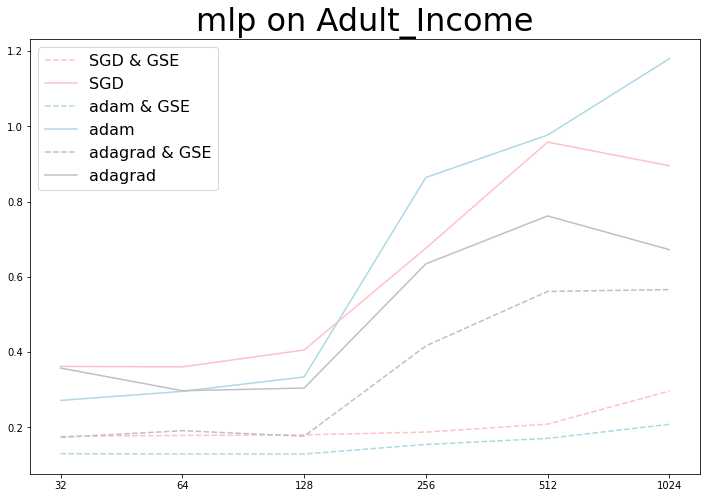
\includegraphics[width=0.7\linewidth]{figures/AdultIncomelossResults.png}
  \caption{Results on the ACI dataset. The dashed curves represents experiments wit \tecnameAbrv  and shows an improvement on the loss for every optimizer used.}
  \label{fig:ACIresults}
\end{figure}


% On top that, we clearly see that \tecname leads to greater variance in our results. Our intuition on it is that we estimate the gradient with less observation as written on line 17 ( $\rhd$ \textcolor{blue}{scaled gradient} ) of Algorithm \ref{alg:DivideByTheGood}.



% \section{Results and Discussion}\label{Results}

% \begin{itemize}
%     \item Maxime \ok ? \no ?
%     \item Thierry \ok ? \no ?
%     \item Victor \ok ? \no ?
% \end{itemize}

% \subsection{Results on \catmod}
% \vline

% To implement our idea on a simple linear regression we worked on the Chicago taxi rides dataset that can be found here \footnote{\url{https://data.cityofchicago.org/Transportation/Taxi-Trips/wrvz-psew}}.

% For each ride, we use the taxi identifier, distance, payment type and the tips amount. 
% We use modified version of linear regression to predict the tip based on the trip distance and the payment type.
% \begin{equation*}\label{eq:naiveModel}
%     tips = a \times distance + b 
% \end{equation*}
% We used a symbolic version of this model where the slope depends on the taxi and the payment method, the intercept remains shared among all the trips:
% \begin{equation*}\label{eq:otherModel}
%     tips = (\gamma_{\text{taxi}} \times \mu_{\text{payment}}) \times distance + b 
% \end{equation*}
% There is one $\gamma$ per taxi and one $\mu$ per payment method, this is a \catmod. As the intercept is shared among all taxis, the dataset is unsplitable. A model $$tips = \gamma_{\text{taxi}}  \times distance + b_{taxi} $$ could be split in different dataset (one per taxi) and thus we would be in the classical setting of a linear regression.

% The relational batch performed better with our proposition based on Algorithm \ref{alg:DivideByTheGood} with the following setting: 30 epochs ; optimizer Adam with default setting ; batch size of 1. Experiment was reproduced 20 times. The used metric is the mean square error (MSE).

% We ran the same experiments on the Belarus used cars dataset.    It is presented presented by \cite{UsedCars} and contains vehicle features. We take into account the car manufacturer, the production year, the origin region of the car to predict the selling price of the car.
% \begin{equation*}\label{eq:otherModelUsedCars}
%     price = (\gamma_{\text{manufacturer}} \times \mu_{\text{region}}) \times year + b 
% \end{equation*}


% \begin{table}[hb!]% h asks to places the floating element [h]ere.
%   \caption{Results with \catmod }
%   \label{tab:envisionResult}
%   \begin{footnotesize}
%   \begin{center}
%   \begin{tabular}{l|cc}
%     \toprule
%     Dataset      & Adam         & Adam \& \tecnameAbrv       \\
%     \midrule                                                                                     
%     Chicago Ride & 35.58 $\pm$ 1.11 & \bold{9.45 $\pm$ 16.33} \\
%     Used Cars & 7.10 $\pm$ 2.45 & \textbf{0.08 $\pm$ 0.01} \\
%   \bottomrule
% \end{tabular}
% \end{center}
% \end{footnotesize}
% \end{table}


% \subsection{Results on \catmod on a real case}


% \TODO validate it with Joannes/Victor

% We have successfully deployed to production such \catmod at Lokad in order to weekly forecast sales of a large retail company. The forecast is done at the item level. The dataset contains 3 years of history and concerns more than $13$ millions different items.

% The implemented \catmod is similar\footnote{we do not disclose the actual model for confidentiality reasons} to:

% %%\begin{equation*}
% \begin{align*}
%     \hat{y}(item, week) = \quad &\theta_{store(item)} \times \theta_{color(item)} \times \theta_{size(item)} \times\\
%       & \Theta [group(item), WeekNumber(week)]
% \end{align*}
% %%\end{equation*}

% $\Theta [group(item), WeekNumber(week)]$ is a parameter vector that can be seen as a function:
% \begin{equation*}
%     \Theta : Groups \times [| 1, 52|] \longrightarrow \mathbb{R}
% \end{equation*}

% It aims to capture the annual seasonality for a given group of items.


% We use Adam with \tecname and a minibatch of $1$ to update the parameters. It outstandingly outperform the classical gradient estimator on this (very) \catmod. 

% \subsection{\ohe Deep Learning}

% To implement our idea on neural networks we worked on 5 different symbolic datasets. 

% \begin{itemize}
%     \item the Adult Census Income (ACI) dataset presented in \cite{incomeDataset} that aims to predict wealth category of individuals.
%     \item the Compas dataset contains symbolic information on criminal defendant’s likelihood of re-offending.
    
%     \item the Don't Get Kicked (DGK) dataset introduced by \cite{DGK}. The objective is to predict if the car purchased at the Auction is a good or a bad buy.
    
%     \item the Forest Cover dataset presented \cite{ForestCover} contains symbolic characteristics on $30m^2$ forest cells. The objective is to predict the forest cover type. 
%     \item the KDD99 dataset accessible by \cite{KDD99} contains symbolic features such as \textit{protocol_type}, \textit{service} and \textit{flag}.
%     \item a Used Cars datasets from Belarus presented above.
% \end{itemize}



% In order to only measure the impact of the \tecname, we \textit{only} use those symbolic variables in our experiments. Those datasets tasks are quiet easy. As a consequence we use a very small network to highlight our approach. Our network is made of 3 dense layers of sizes $[4,8,4]$ with a batch of size $128$. We also perform experiments on a ResNet-like network that give same results. We use the $l_2$ loss. 
% We have tested three different optimizer with their default settings: SGD (vanilla), Adagrad and Adam.

% Results are reproducible in the repository.


% \begin{remark}
% We use the same ResNet-like network than \cite{RevisitingDeepForTabular}.
% \end{remark}







% \subsection{Results interpretation}
% The results are recorded in Tables \ref{tab:resultsMLP1} \ref{tab:resultsMLP8} \ref{tab:resultsMLP32} \ref{tab:resultsMLP128}  \ref{tab:resultsRESNET1} \ref{tab:resultsRESNET8} \ref{tab:resultsRESNET32} \ref{tab:resultsRESNET128}  in appendices. On the different datasets we have worked on, we always see an improvement of the loss on the testing dataset using the \tecname. This proves the need to specifically handle stochastic gradient on symbolic data. Results in different settings demonstrate the advantage to use \tecname whatever the optimizer. Among other things, AdaGrad tries to handle gradient on sparse data (which includes one-hot encoded data) but we see a clear improvement on that task.


% On top that, we clearly see that \tecname leads to greater variance in our results. Our intuition on it is that we estimate the gradient with less observation as written on line 17 ( $\rhd$ \textcolor{blue}{scaled gradient} ) of Algorithm \ref{alg:DivideByTheGood}.


% \subsection{Similarity with embeddings A METTRE AVANT}
% Our proposed solution, i.e. \tecname on one-hot-encoded data, is very similar to vector embedding. The main difference here is the cardinality of the symbolic features concerned. 

% \subsection{Discussion and future work A FUSIONNER AVEC CONCLUSION} 



% The main significance of this work is to highlight the lack of special treatment for symbolic data. They are unfairly underrepresented on public datasets and machine learning in general. We hope that this work will make researchers to take them more into considerations. And our proposed method combined with \ohe, turns every gradient-compatible model into a \catmod! We've shown it even on neural networks. This thus unlocks correct treatment of symbolic data for all gradient-based models. Moreover our gradient estimator clearly helps convergence when dealing with one-hot encoded data. Indeed this estimator add prior knowledge we have on the data to the gradient, thus the gradient conveys all relevant information, which is the expected behavior.



% In the notation Section \ref{notations} we have defined symbol groups by Equation \ref{eq:symbol}. This ``reverse engineer`` \ohe and there might be a better paradigm in order to tackle symbolic dataset via \catmod; this will be the natural following work of this one.

\section{Conclusions}\label{sec:conclusion}

% \begin{itemize}
%     \item Maxime \ok ? \no ?
%     \item Thierry \ok ? \no ?
%     \item Victor \ok ? \no ?
% \end{itemize}



% And our proposed method combined with \ohe, turns every gradient-compatible model into a \catmod! We've shown it even on neural networks. . Moreover our gradient estimator clearly helps convergence when dealing with one-hot encoded data. Indeed this estimator add prior knowledge we have on the data to the gradient, thus the gradient conveys all relevant information, which is the expected behavior.



% In the notation Section \ref{notations} we have defined symbol groups by Equation \ref{eq:symbol}. This ``reverse engineer`` \ohe and there might be a better paradigm in order to tackle symbolic dataset via \catmod; this will be the natural following work of this one.


This work addresses the issue of using stochastic gradient descent on symbolic data. We have shown how \ohe is needed for interpretable models. \secondContrib  otherwise it leads to incoherent gradient. The proposed gradient estimator solves this problem and rely on the observation that \mainContrib. This thus unlocks correct treatment of symbolic data for all gradient-based models. The code and all the details of the study is mainly open-sourced\footnote{https://github.com/ppmdatix/RelationalBatch} and demonstrates its utility on several datasets. 



The main significance of this work is to highlight the lack of special treatment for symbolic data. They are unfairly underrepresented on public datasets and machine learning in general. We hope that this work will make researchers to take them more into considerations. 




\section*{Acknowledgment}
This work was supported by the University of Rouen and the french company Lokad. We would like to thank Gaëtan Delétoille and Antonio Cifonelli for interesting discussions on the topic. 

\bibliographystyle{elsarticle-harv} 
\bibliography{bib/sample}
%%\newpage
\appendix

% \begin{itemize}
%     \item Maxime \ok ? \no ?
%     \item Thierry \ok ? \no ?
%     \item Victor \ok ? \no ?
% \end{itemize}



%%%%%%%%%%%%%%%%%%%%%%%%%
%%%%%%%%%%%%%%%%%%%%%%%%

\begin{table}[h!]
    \begin{footnotesize}
    \begin{center}
    \begin{tabular}{l|cc:cc:cc}
    \toprule
    Dataset               &   SGD           & SGD \& \tecnameAbrv & Adagrad & Adagrad \& \tecnameAbrv & Adam        & Adam \& \tecnameAbrv \\
    \midrule
    \textbf{ACI         } & 0.36 $\pm$ 0.16 & \textbf{0.18 $\pm$ 0.01} & 0.27 $\pm$ 0.07 & \textbf{0.13 $\pm$ 0.01} & 0.36 $\pm$ 0.16 & 0.17 $\pm$ 0.02 \\ 
    \textbf{compas      } & 0.47 $\pm$ 0.28 & 0.24 $\pm$ 0.01 & 0.60 $\pm$ 0.26 & \textbf{0.08 $\pm$ 0.02} & 0.60 $\pm$ 0.19 & 0.38 $\pm$ 0.12 \\ 
    \textbf{DGK         } \\ 
    \textbf{Forest Cover} & 1.98 $\pm$ 0.01 & \textbf{1.95 $\pm$ 0.01} & 1.98 $\pm$ 0.02 & \textbf{1.40 $\pm$ 0.05} & 1.98 $\pm$ 0.01 & 1.96 $\pm$ 0.01 \\ 
    \textbf{KDD99       } & 3.22 $\pm$ 0.12 & \textbf{0.30 $\pm$ 0.07} & 3.10 $\pm$ 0.13 & \textbf{0.17 $\pm$ 0.02} & 3.15 $\pm$ 0.19 & \textbf{0.55 $\pm$ 0.07} \\ 

    \bottomrule
    \end{tabular}
    \caption{Results with mlp and batch of 32}
    \label{tab:resultsMLP32}
    \end{center}
    \end{footnotesize}
\end{table}


\begin{table}[h!]
    \begin{footnotesize}
    \begin{center}
    \begin{tabular}{l|cc:cc:cc}
    \toprule
    Dataset               &   SGD           & SGD \& \tecnameAbrv & Adagrad & Adagrad \& \tecnameAbrv & Adam        & Adam \& \tecnameAbrv \\
    \midrule
    \textbf{ACI         } & 0.37 $\pm$ 0.07 & \textbf{0.13 $\pm$ 0.01} & 0.42 $\pm$ 0.07 & \textbf{0.13 $\pm$ 0.01} & 0.42 $\pm$ 0.07 & \textbf{0.13 $\pm$ 0.01} \\ 
    \textbf{compas      } & 0.69 $\pm$ 0.27 & \textbf{0.06 $\pm$ 0.01} & 0.65 $\pm$ 0.24 & \textbf{0.01 $\pm$ 0.01} & 0.87 $\pm$ 0.47 & \textbf{0.05 $\pm$ 0.01} \\ 
    \textbf{DGK         } \\ 
    \textbf{Forest Cover} & 2.03 $\pm$ 0.03 & \textbf{1.14 $\pm$ 0.01} & 2.02 $\pm$ 0.03 & \textbf{1.04 $\pm$ 0.01} & 2.01 $\pm$ 0.04 & \textbf{1.06 $\pm$ 0.01} \\ 
    \textbf{KDD99       } & 3.24 $\pm$ 0.06 & \textbf{0.06 $\pm$ 0.01} & 3.19 $\pm$ 0.05 & \textbf{0.05 $\pm$ 0.01} & 3.22 $\pm$ 0.06 & \textbf{0.06 $\pm$ 0.01} \\ 

    \bottomrule
    \end{tabular}
    \caption{Results with resnet and batch of 32}
    \label{tab:resultsRESNET32}
    \end{center}
    \end{footnotesize}
\end{table}


\begin{table}[h!]
    \begin{footnotesize}
    \begin{center}
    \begin{tabular}{l|cc:cc:cc}
    \toprule
    Dataset               &   SGD           & SGD \& \tecnameAbrv & Adagrad & Adagrad \& \tecnameAbrv & Adam        & Adam \& \tecnameAbrv \\
    \midrule
    \textbf{ACI         } & 0.36 $\pm$ 0.17 & \textbf{0.18 $\pm$ 0.01} & 0.30 $\pm$ 0.09 & \textbf{0.13 $\pm$ 0.01} & 0.30 $\pm$ 0.14 & 0.19 $\pm$ 0.08 \\ 
    \textbf{compas      } & 0.52 $\pm$ 0.46 & 0.25 $\pm$ 0.01 & 0.57 $\pm$ 0.27 & \textbf{0.12 $\pm$ 0.05} & 0.67 $\pm$ 0.36 & 0.49 $\pm$ 0.25 \\ 
    \textbf{DGK         } & 0.21 $\pm$ 0.06 & \textbf{0.11 $\pm$ 0.01} & 0.19 $\pm$ 0.06 & \textbf{0.11 $\pm$ 0.01} & 0.20 $\pm$ 0.08 & 0.14 $\pm$ 0.04 \\ 
    \textbf{Forest Cover} & 1.99 $\pm$ 0.02 & 1.97 $\pm$ 0.01 & 1.97 $\pm$ 0.01 & \textbf{1.52 $\pm$ 0.09} & 1.98 $\pm$ 0.01 & 1.96 $\pm$ 0.01 \\ 
    \textbf{KDD99       } & 3.09 $\pm$ 0.18 & \textbf{0.38 $\pm$ 0.08} & 3.12 $\pm$ 0.21 & \textbf{0.17 $\pm$ 0.03} & 3.36 $\pm$ 0.12 & \textbf{0.68 $\pm$ 0.16} \\ 

    \bottomrule
    \end{tabular}
    \caption{Results with mlp and batch of 64}
    \label{tab:resultsMLP64}
    \end{center}
    \end{footnotesize}
\end{table}


\begin{table}[h!]
    \begin{footnotesize}
    \begin{center}
    \begin{tabular}{l|cc:cc:cc}
    \toprule
    Dataset               &   SGD           & SGD \& \tecnameAbrv & Adagrad & Adagrad \& \tecnameAbrv & Adam        & Adam \& \tecnameAbrv \\
    \midrule
    \textbf{ACI         } & 0.35 $\pm$ 0.02 & \textbf{0.14 $\pm$ 0.01} & 0.40 $\pm$ 0.11 & \textbf{0.13 $\pm$ 0.01} & 0.47 $\pm$ 0.11 & \textbf{0.13 $\pm$ 0.01} \\ 
    \textbf{compas      } & 0.65 $\pm$ 0.23 & \textbf{0.08 $\pm$ 0.01} & 0.65 $\pm$ 0.31 & \textbf{0.02 $\pm$ 0.01} & 0.59 $\pm$ 0.20 & \textbf{0.06 $\pm$ 0.01} \\ 
    \textbf{DGK         } & 0.27 $\pm$ 0.11 & \textbf{0.12 $\pm$ 0.01} & 0.28 $\pm$ 0.04 & \textbf{0.10 $\pm$ 0.01} & 0.30 $\pm$ 0.13 & \textbf{0.12 $\pm$ 0.01} \\ 
    \textbf{Forest Cover} & 2.02 $\pm$ 0.03 & \textbf{1.29 $\pm$ 0.02} & 2.02 $\pm$ 0.03 & \textbf{1.05 $\pm$ 0.01} & 2.02 $\pm$ 0.03 & \textbf{1.07 $\pm$ 0.01} \\ 
    \textbf{KDD99       } & 3.19 $\pm$ 0.10 & \textbf{0.06 $\pm$ 0.01} & 3.16 $\pm$ 0.08 & \textbf{0.05 $\pm$ 0.01} & 3.23 $\pm$ 0.06 & \textbf{0.06 $\pm$ 0.01} \\ 

    \bottomrule
    \end{tabular}
    \caption{Results with resnet and batch of 64}
    \label{tab:resultsRESNET64}
    \end{center}
    \end{footnotesize}
\end{table}


\begin{table}[h!]
    \begin{footnotesize}
    \begin{center}
    \begin{tabular}{l|cc:cc:cc}
    \toprule
    Dataset               &   SGD           & SGD \& \tecnameAbrv & Adagrad & Adagrad \& \tecnameAbrv & Adam        & Adam \& \tecnameAbrv \\
    \midrule
    \textbf{ACI         } & 0.41 $\pm$ 0.20 & \textbf{0.18 $\pm$ 0.01} & 0.33 $\pm$ 0.18 & \textbf{0.13 $\pm$ 0.01} & 0.30 $\pm$ 0.14 & 0.18 $\pm$ 0.02 \\ 
    \textbf{compas      } & 0.65 $\pm$ 0.19 & \textbf{0.31 $\pm$ 0.03} & 0.56 $\pm$ 0.35 & \textbf{0.12 $\pm$ 0.05} & 0.51 $\pm$ 0.24 & 0.43 $\pm$ 0.19 \\ 
    \textbf{DGK         } \\ 
    \textbf{Forest Cover} & 2.00 $\pm$ 0.02 & 1.98 $\pm$ 0.01 & 1.99 $\pm$ 0.01 & \textbf{1.57 $\pm$ 0.09} & 1.99 $\pm$ 0.02 & 1.97 $\pm$ 0.02 \\ 
    \textbf{KDD99       } & 3.19 $\pm$ 0.14 & \textbf{0.60 $\pm$ 0.19} & 3.27 $\pm$ 0.17 & \textbf{0.16 $\pm$ 0.03} & 3.25 $\pm$ 0.16 & \textbf{0.96 $\pm$ 0.29} \\ 

    \bottomrule
    \end{tabular}
    \caption{Results with mlp and batch of 128}
    \label{tab:resultsMLP128}
    \end{center}
    \end{footnotesize}
\end{table}


\begin{table}[h!]
    \begin{footnotesize}
    \begin{center}
    \begin{tabular}{l|cc:cc:cc}
    \toprule
    Dataset               &   SGD           & SGD \& \tecnameAbrv & Adagrad & Adagrad \& \tecnameAbrv & Adam        & Adam \& \tecnameAbrv \\
    \midrule
    \textbf{ACI         } & 0.78 $\pm$ 0.20 & \textbf{0.14 $\pm$ 0.01} & 0.99 $\pm$ 0.33 & \textbf{0.13 $\pm$ 0.01} & 0.90 $\pm$ 0.22 & \textbf{0.13 $\pm$ 0.01} \\ 
    \textbf{compas      } & 0.69 $\pm$ 0.34 & \textbf{0.11 $\pm$ 0.01} & 0.75 $\pm$ 0.28 & \textbf{0.02 $\pm$ 0.01} & 0.75 $\pm$ 0.53 & \textbf{0.06 $\pm$ 0.01} \\ 
    \textbf{DGK         } \\ 
    \textbf{Forest Cover} & 2.02 $\pm$ 0.03 & \textbf{1.52 $\pm$ 0.03} & 2.01 $\pm$ 0.03 & \textbf{1.03 $\pm$ 0.01} & 2.01 $\pm$ 0.02 & \textbf{1.06 $\pm$ 0.01} \\ 
    \textbf{KDD99       } & 3.18 $\pm$ 0.03 & \textbf{0.07 $\pm$ 0.01} & 3.21 $\pm$ 0.08 & \textbf{0.05 $\pm$ 0.01} & 3.18 $\pm$ 0.07 & \textbf{0.06 $\pm$ 0.01} \\ 

    \bottomrule
    \end{tabular}
    \caption{Results with resnet and batch of 128}
    \label{tab:resultsRESNET128}
    \end{center}
    \end{footnotesize}
\end{table}


\begin{table}[h!]
    \begin{footnotesize}
    \begin{center}
    \begin{tabular}{l|cc:cc:cc}
    \toprule
    Dataset               &   SGD           & SGD \& \tecnameAbrv & Adagrad & Adagrad \& \tecnameAbrv & Adam        & Adam \& \tecnameAbrv \\
    \midrule
    \textbf{ACI         } & 0.68 $\pm$ 0.36 & \textbf{0.19 $\pm$ 0.01} & 0.86 $\pm$ 0.43 & \textbf{0.15 $\pm$ 0.01} & 0.63 $\pm$ 0.43 & 0.42 $\pm$ 0.30 \\ 
    \textbf{compas      } & 0.86 $\pm$ 0.40 & 0.49 $\pm$ 0.15 & 0.57 $\pm$ 0.30 & \textbf{0.20 $\pm$ 0.04} & 0.53 $\pm$ 0.29 & 0.47 $\pm$ 0.24 \\ 
    \textbf{DGK         } \\ 
    \textbf{Forest Cover} & 1.98 $\pm$ 0.02 & 1.97 $\pm$ 0.01 & 1.99 $\pm$ 0.02 & \textbf{1.74 $\pm$ 0.06} & 1.99 $\pm$ 0.02 & 1.97 $\pm$ 0.02 \\ 
    \textbf{KDD99       } & 3.12 $\pm$ 0.18 & \textbf{0.96 $\pm$ 0.22} & 3.11 $\pm$ 0.20 & \textbf{0.19 $\pm$ 0.03} & 3.14 $\pm$ 0.14 & \textbf{1.47 $\pm$ 0.43} \\ 

    \bottomrule
    \end{tabular}
    \caption{Results with mlp and batch of 256}
    \label{tab:resultsMLP256}
    \end{center}
    \end{footnotesize}
\end{table}


\begin{table}[h!]
    \begin{footnotesize}
    \begin{center}
    \begin{tabular}{l|cc:cc:cc}
    \toprule
    Dataset               &   SGD           & SGD \& \tecnameAbrv & Adagrad & Adagrad \& \tecnameAbrv & Adam        & Adam \& \tecnameAbrv \\
    \midrule
    \textbf{ACI         } & 1.00 $\pm$ 0.28 & \textbf{0.14 $\pm$ 0.01} & 1.10 $\pm$ 0.43 & \textbf{0.12 $\pm$ 0.01} & 0.79 $\pm$ 0.18 & \textbf{0.13 $\pm$ 0.01} \\ 
    \textbf{compas      } & 0.73 $\pm$ 0.31 & \textbf{0.17 $\pm$ 0.01} & 0.69 $\pm$ 0.18 & \textbf{0.03 $\pm$ 0.01} & 0.57 $\pm$ 0.17 & \textbf{0.07 $\pm$ 0.01} \\ 
    \textbf{DGK         } \\ 
    \textbf{Forest Cover} & 2.01 $\pm$ 0.03 & \textbf{1.73 $\pm$ 0.02} & 2.01 $\pm$ 0.03 & \textbf{1.05 $\pm$ 0.01} & 2.03 $\pm$ 0.03 & \textbf{1.09 $\pm$ 0.01} \\ 
    \textbf{KDD99       } & 3.14 $\pm$ 0.08 & \textbf{0.08 $\pm$ 0.01} & 3.20 $\pm$ 0.05 & \textbf{0.05 $\pm$ 0.01} & 3.18 $\pm$ 0.07 & \textbf{0.06 $\pm$ 0.01} \\ 

    \bottomrule
    \end{tabular}
    \caption{Results with resnet and batch of 256}
    \label{tab:resultsRESNET256}
    \end{center}
    \end{footnotesize}
\end{table}


\begin{table}[h!]
    \begin{footnotesize}
    \begin{center}
    \begin{tabular}{l|cc:cc:cc}
    \toprule
    Dataset               &   SGD           & SGD \& \tecnameAbrv & Adagrad & Adagrad \& \tecnameAbrv & Adam        & Adam \& \tecnameAbrv \\
    \midrule
    \textbf{ACI         } & 0.96 $\pm$ 0.58 & \textbf{0.21 $\pm$ 0.02} & 0.98 $\pm$ 0.56 & \textbf{0.17 $\pm$ 0.03} & 0.76 $\pm$ 0.44 & 0.56 $\pm$ 0.35 \\ 
    \textbf{compas      } & 0.64 $\pm$ 0.36 & 0.46 $\pm$ 0.20 & 0.51 $\pm$ 0.36 & 0.28 $\pm$ 0.15 & 0.68 $\pm$ 0.35 & 0.63 $\pm$ 0.32 \\ 
    \textbf{DGK         } & 0.19 $\pm$ 0.06 & 0.15 $\pm$ 0.04 & 0.16 $\pm$ 0.06 & 0.11 $\pm$ 0.01 & 0.21 $\pm$ 0.12 & 0.18 $\pm$ 0.09 \\ 
    \textbf{Forest Cover} & 1.98 $\pm$ 0.02 & 1.98 $\pm$ 0.01 & 1.98 $\pm$ 0.02 & \textbf{1.85 $\pm$ 0.05} & 1.99 $\pm$ 0.02 & 1.98 $\pm$ 0.02 \\ 
    \textbf{KDD99       } & 3.17 $\pm$ 0.19 & \textbf{1.11 $\pm$ 0.24} & 3.10 $\pm$ 0.10 & \textbf{0.21 $\pm$ 0.02} & 3.11 $\pm$ 0.18 & \textbf{1.93 $\pm$ 0.41} \\ 

    \bottomrule
    \end{tabular}
    \caption{Results with mlp and batch of 512}
    \label{tab:resultsMLP512}
    \end{center}
    \end{footnotesize}
\end{table}


\begin{table}[h!]
    \begin{footnotesize}
    \begin{center}
    \begin{tabular}{l|cc:cc:cc}
    \toprule
    Dataset               &   SGD           & SGD \& \tecnameAbrv & Adagrad & Adagrad \& \tecnameAbrv & Adam        & Adam \& \tecnameAbrv \\
    \midrule
    \textbf{ACI         } & 0.40 $\pm$ 0.08 & \textbf{0.15 $\pm$ 0.01} & 0.34 $\pm$ 0.04 & \textbf{0.12 $\pm$ 0.01} & 0.38 $\pm$ 0.08 & \textbf{0.13 $\pm$ 0.01} \\ 
    \textbf{compas      } & 0.58 $\pm$ 0.14 & \textbf{0.23 $\pm$ 0.02} & 0.51 $\pm$ 0.12 & \textbf{0.04 $\pm$ 0.01} & 0.62 $\pm$ 0.20 & \textbf{0.07 $\pm$ 0.01} \\ 
    \textbf{DGK         } & 0.26 $\pm$ 0.04 & \textbf{0.17 $\pm$ 0.01} & 0.27 $\pm$ 0.06 & \textbf{0.12 $\pm$ 0.01} & 0.29 $\pm$ 0.08 & \textbf{0.13 $\pm$ 0.01} \\ 
    \textbf{Forest Cover} & 2.02 $\pm$ 0.03 & \textbf{1.86 $\pm$ 0.03} & 2.02 $\pm$ 0.04 & \textbf{1.04 $\pm$ 0.01} & 1.99 $\pm$ 0.04 & \textbf{1.08 $\pm$ 0.01} \\ 
    \textbf{KDD99       } & 3.23 $\pm$ 0.09 & \textbf{0.10 $\pm$ 0.01} & 3.20 $\pm$ 0.08 & \textbf{0.06 $\pm$ 0.01} & 3.23 $\pm$ 0.06 & \textbf{0.07 $\pm$ 0.01} \\ 

    \bottomrule
    \end{tabular}
    \caption{Results with resnet and batch of 512}
    \label{tab:resultsRESNET512}
    \end{center}
    \end{footnotesize}
\end{table}


\begin{table}[h!]
    \begin{footnotesize}
    \begin{center}
    \begin{tabular}{l|cc:cc:cc}
    \toprule
    Dataset               &   SGD           & SGD \& \tecnameAbrv & Adagrad & Adagrad \& \tecnameAbrv & Adam        & Adam \& \tecnameAbrv \\
    \midrule
    \textbf{ACI         } & 0.90 $\pm$ 0.57 & 0.30 $\pm$ 0.09 & 1.18 $\pm$ 0.54 & \textbf{0.21 $\pm$ 0.04} & 0.67 $\pm$ 0.49 & 0.57 $\pm$ 0.44 \\ 
    \textbf{compas      } & 0.56 $\pm$ 0.31 & 0.47 $\pm$ 0.22 & 0.56 $\pm$ 0.21 & 0.42 $\pm$ 0.20 & 0.68 $\pm$ 0.33 & 0.64 $\pm$ 0.31 \\ 
    \textbf{DGK         } & 0.18 $\pm$ 0.09 & 0.15 $\pm$ 0.05 & 0.25 $\pm$ 0.14 & 0.16 $\pm$ 0.07 & 0.18 $\pm$ 0.07 & 0.16 $\pm$ 0.05 \\ 
    \textbf{Forest Cover} & 1.98 $\pm$ 0.02 & 1.98 $\pm$ 0.02 & 1.99 $\pm$ 0.02 & \textbf{1.93 $\pm$ 0.02} & 1.99 $\pm$ 0.02 & 1.98 $\pm$ 0.02 \\ 
    \textbf{KDD99       } & 3.29 $\pm$ 0.13 & \textbf{1.66 $\pm$ 0.34} & 3.16 $\pm$ 0.15 & \textbf{0.21 $\pm$ 0.02} & 3.09 $\pm$ 0.11 & \textbf{2.40 $\pm$ 0.21} \\ 

    \bottomrule
    \end{tabular}
    \caption{Results with mlp and batch of 1024}
    \label{tab:resultsMLP1024}
    \end{center}
    \end{footnotesize}
\end{table}


\begin{table}[h!]
    \begin{footnotesize}
    \begin{center}
    \begin{tabular}{l|cc:cc:cc}
    \toprule
    Dataset               &   SGD           & SGD \& \tecnameAbrv & Adagrad & Adagrad \& \tecnameAbrv & Adam        & Adam \& \tecnameAbrv \\
    \midrule
    \textbf{ACI         } & 0.48 $\pm$ 0.14 & \textbf{0.18 $\pm$ 0.01} & 0.39 $\pm$ 0.05 & \textbf{0.13 $\pm$ 0.01} & 0.42 $\pm$ 0.11 & \textbf{0.13 $\pm$ 0.01} \\ 
    \textbf{compas      } & 0.59 $\pm$ 0.16 & \textbf{0.27 $\pm$ 0.01} & 0.60 $\pm$ 0.19 & \textbf{0.05 $\pm$ 0.01} & 0.72 $\pm$ 0.30 & \textbf{0.09 $\pm$ 0.02} \\ 
    \textbf{DGK         } & 0.29 $\pm$ 0.07 & \textbf{0.18 $\pm$ 0.01} & 0.25 $\pm$ 0.05 & \textbf{0.12 $\pm$ 0.01} & 0.30 $\pm$ 0.13 & \textbf{0.13 $\pm$ 0.01} \\ 
    \textbf{Forest Cover} & 2.00 $\pm$ 0.03 & \textbf{1.91 $\pm$ 0.03} & 2.02 $\pm$ 0.03 & \textbf{1.09 $\pm$ 0.01} & 2.00 $\pm$ 0.03 & \textbf{1.14 $\pm$ 0.01} \\ 
    \textbf{KDD99       } & 3.19 $\pm$ 0.09 & \textbf{0.13 $\pm$ 0.01} & 3.17 $\pm$ 0.05 & \textbf{0.05 $\pm$ 0.01} & 3.18 $\pm$ 0.05 & \textbf{0.07 $\pm$ 0.01} \\ 

    \bottomrule
    \end{tabular}
    \caption{Results with resnet and batch of 1024}
    \label{tab:resultsRESNET1024}
    \end{center}
    \end{footnotesize}
\end{table}
%%%%%%%%%%%%%%%%%%%%%%%%%%%%%%
%%%%%%%%%%%%%%%%%%%%%%%%%%%%%%


\subsection{Performance impact}
To implement this solution, we need to count each symbol occurrence in the batch. If well implemented, this is negligible. Especially when the data is column-oriented, you only need to \textit{group by} symbol and count them. Moreover this has no relationship with the $\theta$'s value, it can be pre-computed and reused at every epoch if the training dataset stay static through steps.




%%%%%%%%%%%%%%%%%%%%%%%%%
%%%%%%%%%%%%%%%%%%%%%%%%

\section{Uniform draw}\label{tirage}

Let $Z$ be a non-empty finite set and $T \subset Z$ also non empty.

We uniformly draw $m > 0$ elements in $Z$ with replacement. We focus on the first drawing where at least one of the $m$ drawn elements belongs to $T$. We note $\Tilde{K}$ this drawing. Thus:

\begin{align}
    \mathbb{P}(\Tilde{K} = 1) &= 1 - (\frac{\abs{Z}-\abs{T}}{\abs{Z}})^m = P_1\\
    \mathbb{P}(\Tilde{K} = n) &= (1 - P_1)^{n-1} P_1
\end{align}

\begin{theorem}[Stoping time]\label{theorem:stop}
$\esp{\Tilde{K}} = \frac{1}{P_1}$
\end{theorem}



\begin{proof}
\begin{align*}
    \esp{\Tilde{K}} = \sum_{n = 1}^{N} n \mathbb{P}(\Tilde{K} = n) &= \sum_{n = 1}^{N} n (1 - P_1)^{n-1} P_1\\
    &= \frac{P_1}{1 - P_1} \sum_{n = 1}^{N} n  (1 - P_1)^{n} 
\end{align*}

For $ 0 < x < 1$  we get:

\begin{align*}
    \sum_{n = 1}^{\infty} n x^n &= \sum_{n = 1}^{\infty} x \frac{\partial x^n}{\partial x}\\
                                &= x \frac{\partial }{\partial x} \sum_{n = 1}^{\infty} x^n\\
                                &= x \frac{\partial }{\partial x} \sum_{n = 0}^{\infty} x^n\\
                                &= x \frac{\partial }{\partial x} \frac{1}{1-x}\\
                                &= \frac{x}{(1-x)^2}
\end{align*}

Then 

\begin{align*}
    \sum_{n = 1}^{\infty} n \mathbb{P}(\Tilde{K} = n) &= \frac{P_1}{1 - P_1} \frac{1-P_1}{P_{1}^2}\\
    &= \frac{1}{P_1}
\end{align*}
\end{proof}

\begin{remark}
It is the same result if the drawings are done without replacement. The only difference is a highest $P_1$.
\end{remark}
\section{Estimator}



Let $Z$ be a non-empty finite set and $T \subset Z$ also non empty.

We have a score function $s$ on $T$:

\begin{equation*}
\begin{split}
    s \quad : \quad &T \longrightarrow \mathbb{R}\\
    &t                 \longrightarrow s(t)
\end{split}
\end{equation*}



We aim to estimate 
\begin{equation*}
    s_T = \frac{1}{\abs{T}} \sum_{x \in T} s(x)
\end{equation*}

Let $(M_k)_{k \leq K}$ a serie of $K$ draws uniform with replacement of $m$ elements of $Z$.

\begin{remark}\label{rem:K>1}
    Thanks to Theorem \ref{theorem:stop} we can ignore the first draws $M_{0}$ such as $M_{0} \cap T = \emptyset$
\end{remark}

One notes


\begin{align*}
    M_k &= (M_k \cap T ) \sqcup (M_k \cap (Z \backslash T)) \\
        &= (M_k^T ) \sqcup (M_k \cap (Z \backslash T))
\end{align*}

\[
   avg(M_k^T) = 
\begin{cases}
     \quad 0 \quad \text{if} \quad M_k^T  = \emptyset\\
    \frac{1}{\abs{M_k^T}} \sum_{x \in M_k^T}s(x) \quad \text{otherwise}
\end{cases}
\]
and

\begin{equation*}
    \bar{K} = \abs{ \{ k \leq K | M_k^T \neq \emptyset \}}
\end{equation*}

Thanks to Remark \ref{rem:K>1} we have $\bar{K} \geq 1$. Then the proposed estimator is $\hat{a}$:

\begin{equation*}
    \hat{a} = \frac{1}{\bar{K}} \sum_{k = 1}^{K}avg(M_k^T)
\end{equation*}



\begin{theorem}[Unbiased estimator]\label{theorem:unbiased}
$\hat{a}$ is an unbiased estimator of $s_T$
\end{theorem}



\begin{proof}
\begin{align*}
    \esp{\Tilde{a}} &= \frac{1}{\hat{K}} \sum_{\underset{k = 1}{M_k^T \neq \emptyset}}^{K} \frac{1}{\abs{(M_k^T)}} \sum_{x \in M_k^T} \esp{s(x)}\\
    &= \frac{\bar{K}}{\bar{K}} \frac{\abs{M_k^T}}{\abs{M_k^T}} \esp{s_T}\\
    &= s_T
\end{align*}
\end{proof}
\end{document}
\endinput